\chapter{Predicting susceptibility to tuberculosis based on gene expression profiling}\label{ch:tb-suscept}

\section[Abstract]{Abstract\footnotemark}

Tuberculosis is a deadly infectious disease, which kills millions of
people every year. The causative pathogen, \emph{Mycobacterium
  tuberculosis} (MTB), is estimated to have infected up to a third of
the world's population; however, only approximately 10\% of healthy
individuals progress to active TB disease. Despite evidence for
heritability, it is not currently possible to predict whether a
healthy person is susceptible to TB. To explore approaches to classify
susceptibility to TB, we infected dendritic cells (DCs) from
individuals known to be susceptible or resistant to TB with MTB, and
measured genome-wide gene expression levels in infected and uninfected
cells. We found hundreds of differentially expressed genes between
susceptible and resistant individuals in the non-infected cells. We
further found that genetic polymorphisms in proximity to the
differentially expressed genes between susceptible and resistant
individuals are more likely to be associated with TB susceptibility in
published GWAS data. In particular, we identified two promising
candidate genes: \emph{CCL1} and \emph{UNC13A}. Lastly, we trained a
classifier based on the gene expression levels in the non-infected
cells, and demonstrated decent performance on our data and an
independent data set. Overall, our promising results from this small
study suggest that training a classifier on a larger cohort may enable
us to accurately predict TB susceptibility.

\footnotetext{Citation for chapter: John D Blischak*, Ludovic
  Tailleux*, Marsha Myrthil, Luis B Barreiro, and Yoav
  Gilad. Predicting susceptibility to tuberculosis based on gene
  expression profiling. In preparation. * denotes equal contribution.}

\section{Introduction}\label{ch03-introduction}

Tuberculosis (TB) is a major public health issue. Worldwide, over a
million people die of TB annually, and millions more currently live
with the disease \citep{WHO2015a, WHO2015b, Glaziou2015}. Successful
treatment requires months of antibiotic therapy \citep{Sotgiu2015},
and the difficulty of adhering to the full treatment regimen has lead
to the emergence of drug-resistant strains of \emph{Mycobacterium
  tuberculosis} (MTB) \citep{Seung2015}.

Approximately a third of the world's population has been infected with
MTB, but most are asymptomatic. While these naturally resistant
individuals are able to avoid active disease, MTB persists in a
dormant state inside their innate immune cells, known as a latent TB
infection \citep{Munoz2015}. In contrast, approximately 10\% of
individuals will develop active TB after infection with MTB
\citep{North2004, OGarra2013}. Unfortunately, we are currently unable
to predict if an individual is susceptible. While twin and family
studies have indicated a heritable component of TB susceptibility
\citep{Kallmann1943, Comstock1978, Cobat2010, Moller2010}, genome wide
association studies (GWAS) have only identified a few loci with low
effect size \citep{Thye2010, Mahasirimongkol2012, Thye2012, Png2012,
  Chimusa2014, Curtis2015, Sobota2016}. Due to the highly polygenic
architecture, it may be informative to examine differences between
susceptible and resistant individuals at a higher level of
organization, e.g. gene regulatory networks. Using this approach,
previous studies have characterized gene expression profiles in innate
immune cells isolated from individuals known to be susceptible or
resistant to infectious diseases, including tuberculosis
\citep{Thuong2008} and acute rheumatic fever \citep{Bryant2014}.

We hypothesized that gene expression profiles in innate immune cells
may be used to classify individuals with respect to their
susceptibility to develop an active TB infection. To test this
hypothesis, we isolated innate immune cells from individuals that are
resistant or susceptible to TB and infected them with MTB. We
discovered that the gene expression differences between resistant and
susceptible innate immune cells were present primarily in the
non-infected state, that these differentially expressed genes were
enriched for nearby SNPs with low p-values in TB susceptibility GWAS,
and furthermore, that these gene expression levels could be used to
classify individuals based on their susceptibility status.

\section{Results}

\subsection{Susceptible individuals have an altered transcriptome in the non-infected state}

We obtained whole blood samples from 25 healthy individuals
(Supplementary Table \ref{ch03-s1}). Six of the donors had recovered
from a previous active TB infection, and are thus susceptible. The
remaining 19 tested positive for a latent TB infection without ever
experiencing symptoms of active TB, and are thus resistant. We
isolated dendritic cells (DCs) and treated them with
\emph{Mycobacterium }\emph{tuberculosis} (MTB) or a mock control for
18 hours. To measure genome-wide gene expression levels in infected
and non-infected samples, we isolated and sequenced RNA using a
processing pipeline designed to minimize the introduction of unwanted
technical variation (Supplementary Fig. \ref{fig:process}). We
obtained a mean ($\pm$ SEM) of 48 $\pm$ 6 million raw reads per
sample. We performed quality control analyses to remove non-expressed
genes (Supplementary Fig.  \ref{fig:gene}; Supplementary Table
\ref{ch03-s2}), identify and remove outliers (Supplementary
Fig. \ref{fig:heat-all}, \ref{fig:heat-filt}, \ref{fig:outliers}), and
check for confounding batch effects (Supplementary
Fig. \ref{fig:batch-effect}, \ref{fig:infection}). Ultimately 6
samples failed the quality checks and were removed from all downstream
analyses (Supplementary Fig. \ref{fig:outliers}).

We performed a standard differential expression analysis using a
linear modeling framework (Supplementary Table \ref{ch03-s3}), defined
in equation (\ref{eq:limma}). As expected, there was a strong response
to infection with MTB in both resistant and susceptible individuals
(Supplementary Fig. \ref{fig:limma-supp}). Considering the resistant
individuals, we identified 3,486 differentially expressed (DE) genes
between the non-infected and infected states at a q-value of 10\% and
an arbitrary absolute log-fold change greater than 1. Similarly, 3,789
genes were DE between the non-infected and infected states for
susceptible individuals at a q-value of 10\% and an absolute log fold
change greater than 1. The DE genes included the important immune
response factors \emph{IL12B}, \emph{REL}, and \emph{TNF}. While the
treatment effect was obvious in all individuals, of most interest were
the patterns of gene expression differences between susceptible and
resistant individuals in either the non-infected or infected states
(Fig. \ref{fig:limma}). We identified 645 DE genes between resistant
and susceptible individuals in the non-infected state at a q-value of
10\%, including \emph{ATPV1B2}, \emph{FEZ2}, \emph{PSMA2},
\emph{TNFRSF25}, and \emph{TRIM38}. In contrast, no genes were DE
between resistant and susceptible individuals in the infected state
(q-value of 10\%).

\begin{figure}
\centering 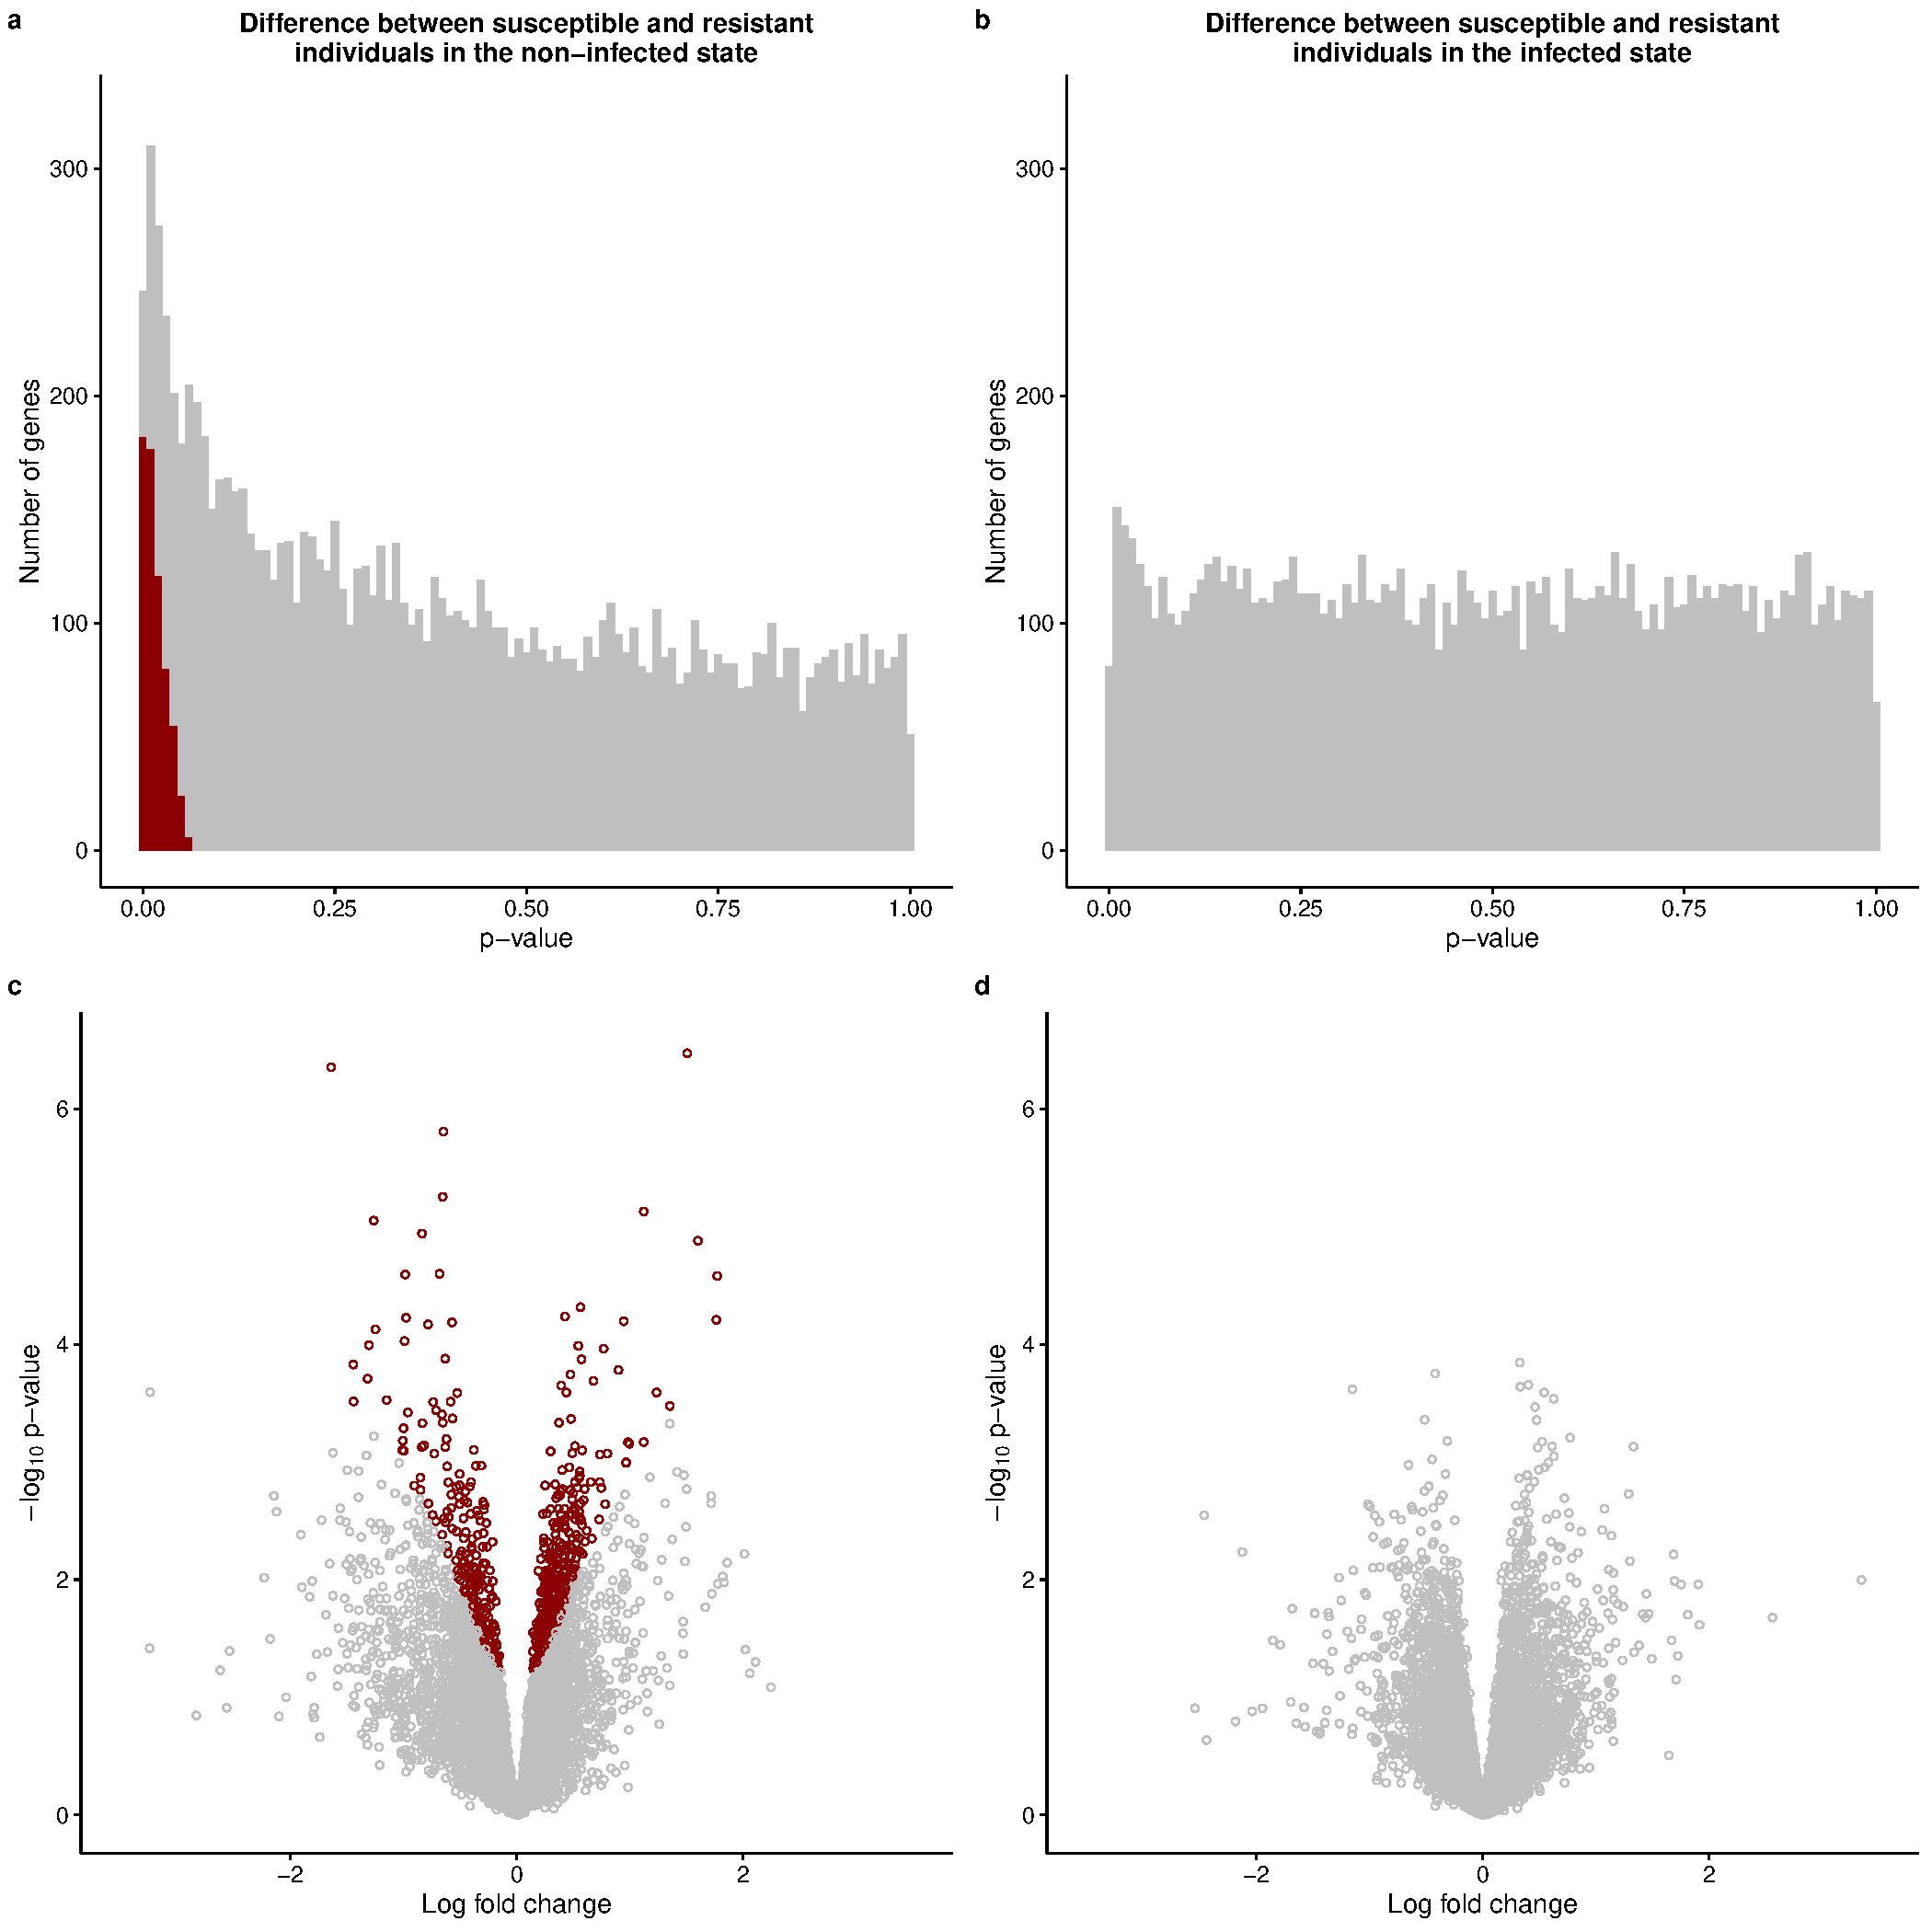
\includegraphics[width=5in]{img/ch03/limma.pdf}
\caption[Differential expression analysis.]{ \textbf{Differential
    expression analysis.} The top panel contains the distribution of
  unadjusted p-values after testing for differential expression
  between susceptible and resistant individuals in the (a)
  non-infected or (b) infected state. The bottom panel contains the
  corresponding volcano plots for the (c) non-infected and (d)
  infected states. The x-axis is the log fold change in gene
  expression level between susceptible and resistant individuals and
  the y-axis is the –log\textsubscript{10} p-value. Red indicates
  genes which are significant differentially expressed with a q-value
  less than 10\%.  }
\label{fig:limma}
\end{figure}
\subsection{Differentially expressed genes are enriched with TB susceptibility loci}

We next sought evidence that genes classified as DE in our \emph{in
  vitro} experimental system play a role in determining susceptibility
to TB. To do this, we intersected our results with those from a TB
susceptibility GWAS conducted in The Gambia and Ghana
\citep{Thye2010}.  To perform a combined analysis of the both data
sets, we coupled each gene in our expression data with the GWAS SNP
with the lowest p-value among all tested SNPs located within 50 kb of
the gene's transcription start site (Supplementary Table
\ref{ch03-s4}). We then asked whether the GWAS SNPs coupled with the
genes we classified as DE between susceptible and resistant
individuals in our experiment are enriched for low GWAS p-values
compared to SNPs coupled to randomly chosen genes.  Specifically, we
calculated the fraction of SNPs with a GWAS p-value less than 0.05
among SNPs coupled with ranked subsets of genes whose expression
profiles show increasing difference between susceptible and resistant
individuals (the effect size was the absolute value of the log fold
change in our experiment). In order to assess the significance of the
observations, we performed 100 permutations of the enrichment analysis
to derive an empirical p-value (Fig.  \ref{fig:gwas}b). Using this
approach, we observed a clear enrichment (empirical \emph{P} \textless
\, 0.01) of low GWAS p-values for SNPs coupled with the genes
classified as DE between susceptible and resistant individuals
(Fig. \ref{fig:gwas}a). We obtained similar results for the Ghana
GWAS; see Supplementary Fig.  \ref{fig:gwas-supp}).

We used this combined expression and GWAS data set to identify genes
potentially involved in TB susceptibility. Only two genes, \emph{CCL1}
and \emph{UNC13A}, were associated with a p-value less than 0.01 in
both The Gambia and Ghana GWAS and had an absolute log fold change
greater than 2 between susceptible and resistant individuals in the
non-infected state (these arbitrary cutoffs were chosen to be
stringent; see Supplementary Table \ref{ch03-s4} for the results with
various cutoffs). Interestingly, these two genes were previously shown
to play a role in MTB infection.

\begin{figure}
\centering 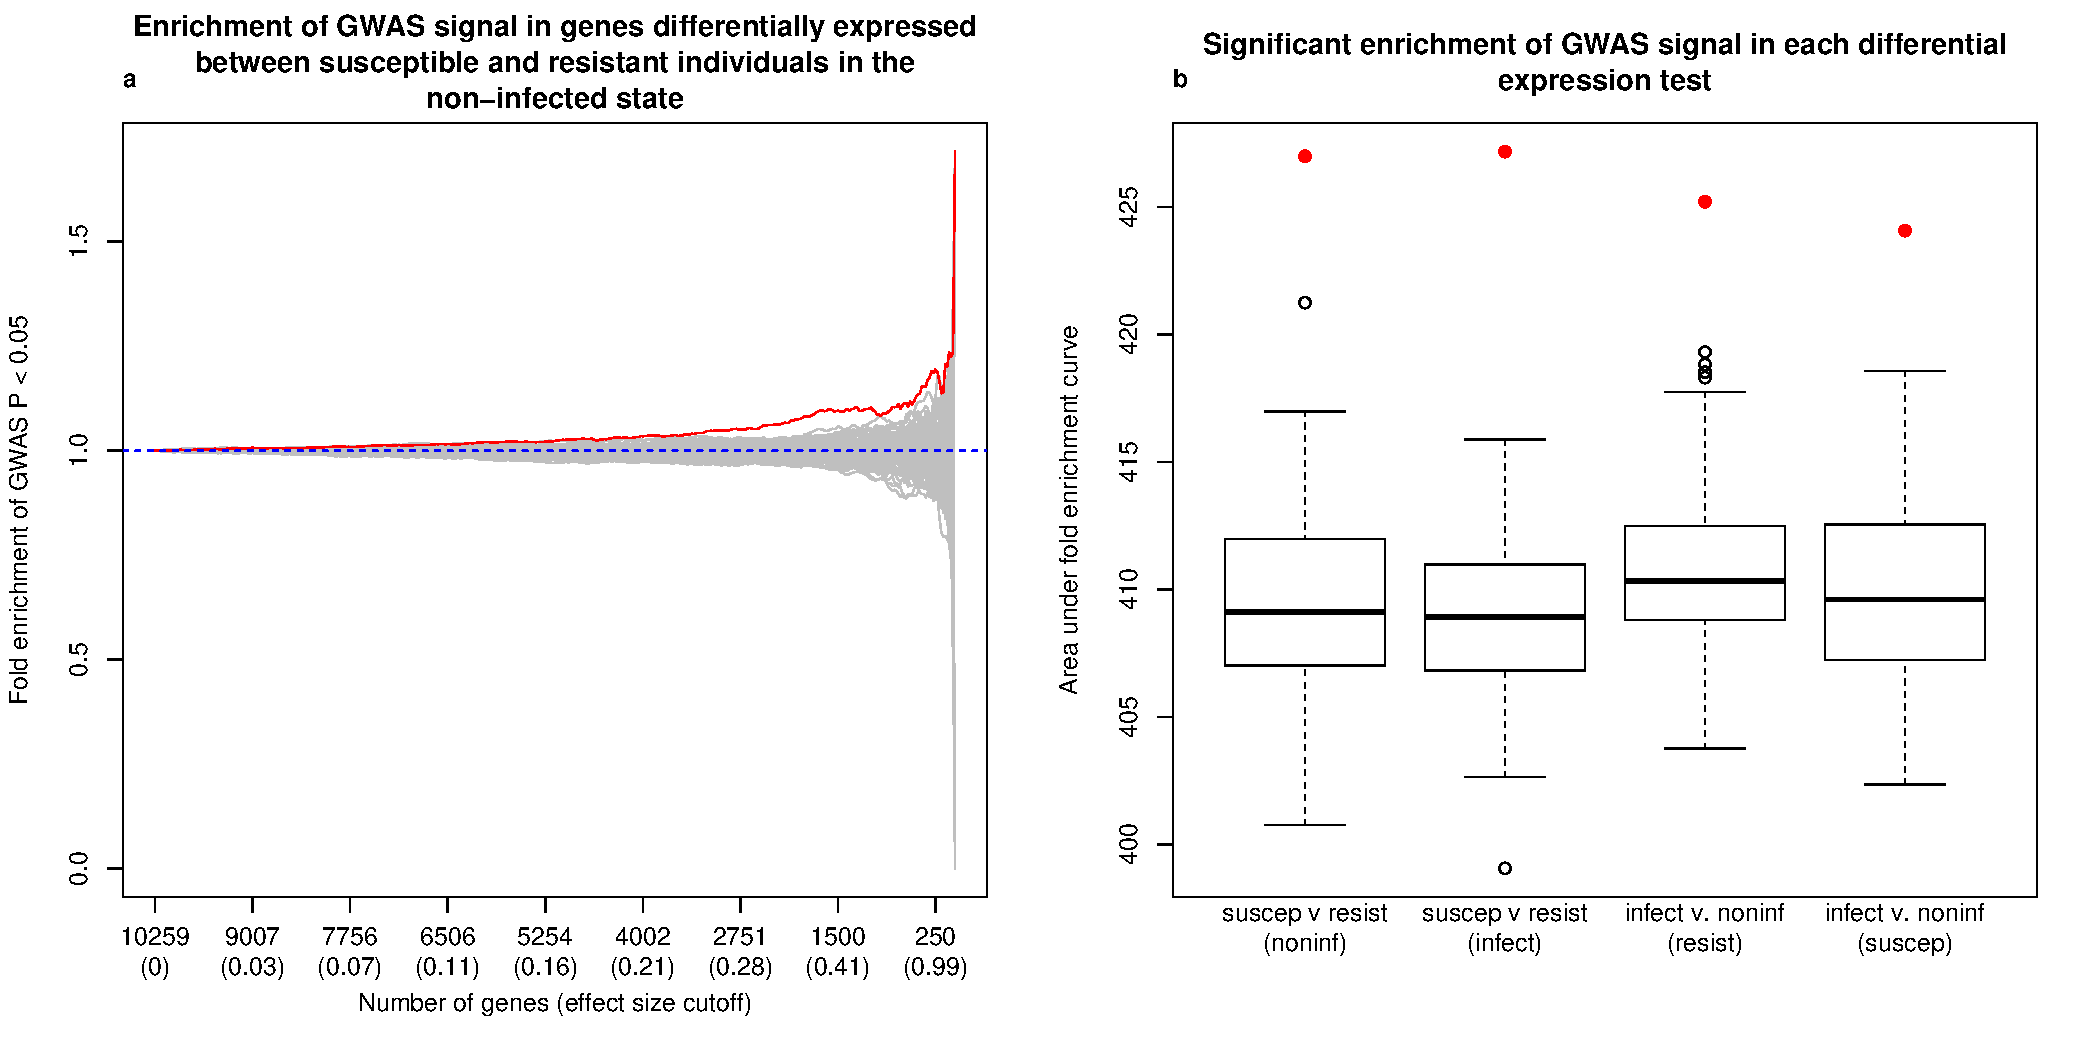
\includegraphics[width=5in]{img/ch03/gwas.pdf}
\caption[Comparison of differential expression and The Gambia GWAS
  results.]{ \textbf{Comparison of differential expression and The
    Gambia GWAS results.} (a) The y-axis is the fold enrichment
  (y-axis) of genes assigned a SNP with p-value less than 0.05 from
  the GWAS in The Gambia \citep{Thye2010}. The x-axis is bins of genes
  with increasingly stringent effect size cutoffs of the absolute log
  fold change between susceptible and resistant individuals in the
  non-infected state. The effect size cutoffs were chosen such that
  each bin from left to right contained approximately 25 fewer
  genes. The red line is the results from the actual data. The grey
  lines are the results from 100 permutations. The dashed blue line at
  y=1 is the null expectation. (b) The x-axis is each of the 4
  differential expression tests performed.  The y-axis is the area
  under the curve of the fold enrichment. The boxplot is the result of
  the 100 permutations, and the red point is the result from the
  actual data. As a reference, the leftmost boxplot corresponds to the
  enrichment plot in (a).  }
\label{fig:gwas}
\end{figure}

\subsection{Susceptibility status can be predicted based on gene expression data}

Next we attempted to build a gene expression-based classifier to
predict TB susceptibility status (Supplementary Table
\ref{ch03-s5}). We focused on the gene expression levels measured in
the non-infected state both because this is where we observed the
largest gene regulatory differences between susceptible and resistant
individuals (Fig.  \ref{fig:limma}ac), and also because, from the
perspective of a translational application, it is more practical to
obtain gene expression data from non-infected DCs. We trained a
support vector machine using the 99 genes that were differentially
expressed between resistant and susceptible individuals in the
non-infected state at a q-value less than 5\% (see Methods for a full
description of how we selected this model). Encouragingly, we observed
a clear separation between susceptible and resistant individuals when
comparing the predicted probability of being resistant to TB for each
sample obtained from leave-one-out-cross-validation (Fig.
\ref{fig:classifier}a). Using a cutoff of 0.75 for the predicted
probability of being resistant to TB, we obtained a sensitivity of
100\% (5 out of 5 susceptible individuals classified as susceptible)
and a specificity of \mytilde88\% (15 out of 17 resistant individuals
were classified as resistant).

Unfortunately our current data set is too small to properly split into
separate training and testing sets (it is challenging to collect
samples from previous TB patients, who are healthy and have no medical
reason to go back for a GP visit). To our knowledge, there are also no
other similar data sets available. Thus, in order to further assess
the plausibility of our model, we applied the classifier to an
independent study, which collected genome-wide gene expression levels
in DCs from 65 healthy individuals \citep{Barreiro2012}, none with a
previous history of TB. Using the cutoff of 0.75 for the probability
of being resistant to TB (determined to be optimal in the training
set), \mytilde11\% (7 of 65) of the individuals were classified as
susceptible to TB. This result is intriguing similar to the estimate
that roughly 10\% of the general population is susceptible to TB
(Fig. \ref{fig:classifier}b).

\begin{figure}
\centering 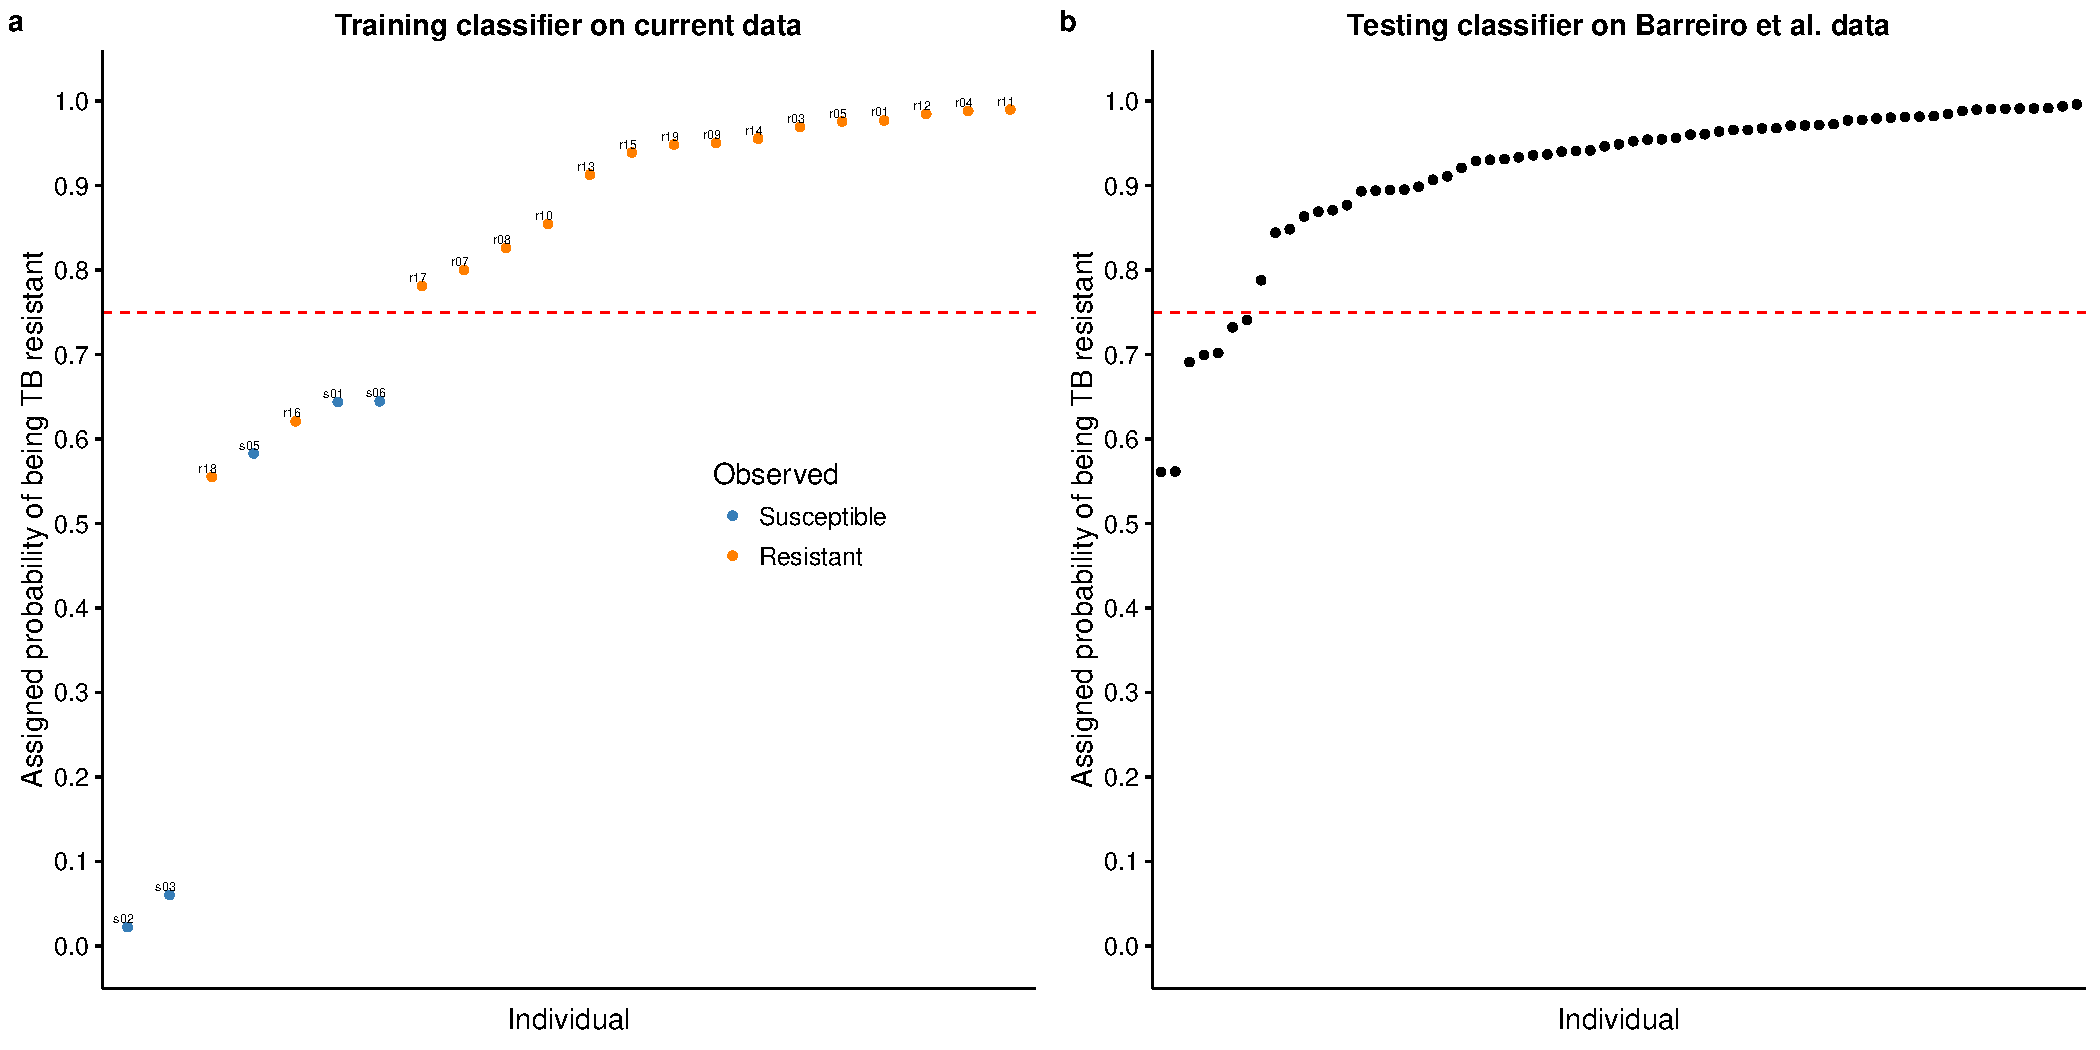
\includegraphics[width=5in]{img/ch03/classifier-svm.pdf}
\caption[Classifying TB susceptible individuals using a support vector
  machine model.]{ \textbf{Classifying TB susceptible individuals
    using a support vector machine model.} (a) The estimates of
  predicted probability of TB resistance from the
  leave-one-out-cross-validation for individuals in the current
  study. The blue circles represent individuals known to be
  susceptible to TB, and orange those resistant to TB. The horizontal
  dashed red line at a probability of 0.75 separates susceptible and
  resistant individuals. (b) The estimates of predicted probability of
  TB resistance from applying the classifier trained on the data from
  the current study to a test set of independently collected healthy
  individuals \citep{Barreiro2012}.  }
\label{fig:classifier}
\end{figure}

\section{Discussion}

We obtained dendritic cells (DCs) from individuals that were known to
be susceptible or resistant to developing active tuberculosis (TB) and
measured genome-wide gene expression levels in non-infected DCs and
DCs infected with \emph{Mycobacterium tuberculosis} (MTB) for 18
hours. As expected, there were large changes in gene expression due to
MTB infection in both resistant and susceptible individuals
(Supplementary Fig. \ref{fig:limma-supp}). We identified 645 genes,
which were differentially expressed (DE) between susceptible and
resistant individuals in the non-infected state; whereas, we did not
observe any DE genes between susceptible and resistant individuals in
the infected state (Fig. \ref{fig:limma}). This suggests that the
differences in the transcriptomes between DCs of resistant and
susceptible individuals are present pre-infection, and affect the
initial response to MTB. Yet, 18 hours after infection gene expression
profiles in both susceptible and resistant individuals have converged
to the same gene regulatory network to fight the active infection. We
chose to measure gene expression 18 hours post-infection because this
time point was previously associated with a large change in
genome-wide gene expression levels \citep{Tailleux2008}. Given our
observations, however, future studies investigating the difference in
the innate immune response between individuals resistant and
susceptible to TB may want to focus on earlier time points post
infection.

Among the 645 DE genes between resistant and susceptible individuals
in the non-infected state, there were many interesting genes involved
in important innate immune activities critical for fighting MTB and
other pathogens such as autophagy \citep{Deretic2014,
  Castrejon-Jimenez2015}, phagolysosomal acidification, and antigen
processing. In particular, \emph{FEZ2}, a suppressor of autophagosome
formation \citep{Spang2014}, was down-regulated when DCs were infected
with MTB; however, in the non-infected DCs, this gene has elevated
expression level in susceptible compared with resistant individuals.
In turn, \emph{ATP6V1B2}, a gene coding for a subunit of the proton
transporter responsible for acidifying phagolysosomes
\citep{Sturgill-Koszycki1994, Hornef2002, Hestvik2005}, has increased
expression in susceptible individuals compared to resistant in the
non-infected state. Lastly, genes coding for nine subunits of the
proteasome, which is critical for processing of MTB antigens to be
presented via major histocompatibility complex (MHC) class I molecules
\citep{Flynn1992, Grotzke2009, Grotzke2010, LindestamArlehamn2014},
have increased expression in susceptible individuals compared to
resistant in the non-infected state. These genes are candidates for
future functional studies investigating the mechanisms of TB
susceptibility.

To our knowledge, our study was only the second to collect data from
\emph{in vitro} MTB infected innate immune cells isolated from
individuals known to be susceptible to MTB (Thuong et al., 2008).
However, there were substantial differences between our study and that
of Thuong et al., 2008 \citep{Thuong2008}. First, they isolated and
infected macrophages, the primary target host cell in which MTB
resides; whereas, we infected DCs, which play a larger role in
stimulating the adaptive immune response to MTB. Second, the
susceptible individuals in Thuong et al., 2008 had an active TB
infection at the time the cells were isolated; whereas, our
individuals had recovered from a past TB infection. Third, we
collected samples from a larger number of resistant individuals (19
versus 4), increasing our power to distinguish between the gene
expression profiles of susceptible and resistant individuals.

We observed that DE genes in our \emph{in vitro} experimental system
were enriched for lower GWAS p-values (Fig. \ref{fig:gwas}). This
suggests that such \emph{in vitro} approaches are informative for
interrogating the genetic basis of disease susceptibility. That being
said, we recognized multiple caveats with this analysis. First,
assigning SNPs to their nearest gene on the linear chromosome is
problematic because regulatory variants can have longer range effects.
Second, the fold enrichments we calculated, albeit statistically
significant, were modest, indicating there were also many SNPs with
low p-values nearby genes with low effect sizes in our experiment. It
is possible that these variants contribute to TB susceptibility by
affecting gene expression in other cell types or environmental
conditions. Third, the individuals in our study were Europeans;
whereas, the GWAS were conducted in Africans. Nevertheless,
considering these limitations, it was encouraging that we were able to
detect evidence of the genetic basis of TB susceptibility in this
system.

Not only did this analysis identify a global enrichment of TB
susceptibility loci, but by intersecting the expression and GWAS data,
we were able to identify two genes (\emph{CCL1} and \emph{UNC13A})
which were marginally significant in both. Interestingly, both of
these genes were previously shown to play important roles in MTB
infection. \emph{CCL1} is a chemokine that stimulates migration of
monocytes \citep{Miller1992}. In our study, it was upregulated in
susceptible individuals compared to resistant in both the non-infected
and infected states (but did not reach statistical significance in
either) and was statistically significantly upregulated with MTB
treatment. The previous differential expression study of TB
susceptibility mentioned above found that \emph{CCL1} was upregulated
to a greater extent 4 hours post MTB-infection in macrophages isolated
from individuals with an active TB infection (i.e. susceptible)
compared to individuals with a latent TB infection (i.e. resistant)
\citep{Thuong2008}. Additionally they performed a candidate gene
association study and found that SNPs nearby \emph{CCL1} were
associated with TB susceptibility. In a previous study from our lab,
we discovered that \emph{CCL1} was one of only 288 genes that were
differentially expressed in macrophages 48 hours post-infection with
MTB and related mycobacterial species but not unrelated virulent
bacteria \citep{Blischak2015}. \emph{UNC13A} is involved in vesicle
formation \citep{Sudhof2004}. In our study, it was downregulated in
susceptible individuals compared to resistant in both the non-infected
and infected states (but did not reach statistical significance in
either) and was statistically significantly upregulated with MTB
treatment. In our past study mapping expression quantitative trait
loci (eQTLs) in DCs 18 hours post-infection with MTB, \emph{UNC13A}
was one of only 98 genes which was associated with an eQTL
post-infection but not pre-infection, which we called an MTB-specific
eQTL \citep{Barreiro2012}. Thus our new results increased the evidence
that \emph{CCL1} and \emph{UNC13A} play important roles in TB
susceptibility.

Previous attempts to use gene expression based classifiers in the
context of TB have focused on predicting the status of an infection
rather than the susceptibility status of an individual
\citep{Berry2010, OGarra2013, Blankley2014}. In other words, the goal
of most previous study was to detect individuals in an early stage of
an active TB infection when antibiotic intervention would be most
effective or to monitor the effectiveness of a treatment regimen
\citep{Maertzdorf2015}. In contrast, our goal was not to distinguish
between an active or latent infection, but instead to be able to
determine susceptibility status before individuals have an active TB
infection. Even with our small sample size, we were able to
successfully train a classier with high sensitivity and decent
specificity. Because such a classification of susceptibility status
could affect the decision of whether or not to take antibiotics to
treat a latent TB infection \citep{Munoz2015}, false negatives
(susceptible individuals mistakenly classified as resistant) would be
much more harmful than false positives (resistant individuals
mistakenly classified as susceptible), which is why we emphasized
sensitivity over specificity.

At this time, we are not aware of any other data set from healthy
individuals known to be sensitive to TB, with which we can further
test our classifier. When we applied our classifier to an independent
set of non-infected DCs isolated from healthy individuals of unknown
susceptibility status, our model predicted that \mytilde11\% of the
individuals were susceptible TB, which reassuringly is similar to the
average in the general population (10\%). Despite this success, our
results must be interpreted cautiously as a proof-of-principle due to
our very small sample size of only 5 susceptible individuals. That
said, our promising results in this small study suggest that
collecting blood samples from a larger cohort of susceptible
individuals would enable building a gene expression based classifier
able to confidently assess risk of TB susceptibility. By reducing the
number of resistant individuals receiving treatment for a latent TB
infection, we can eliminate the adverse health effects of a 6 month
regimen of antibiotics for these individuals and also reduce the
selective pressures on MTB to develop drug resistance.
\section{Methods}

\subsection{Ethics Statement}

We recruited 25 subjects to donate a blood sample for use in our
study. All methods were carried out in accordance with relevant
guidelines and regulations. The experimental protocols were approved
by the Institutional Review Boards of the University of Chicago
(10-504-B) and the Institut Pasteur (IRB00006966). All study
participants provided written informed consent.
\subsection{Sample collection}

We collected whole blood samples from healthy Caucasian male
individuals living in France. The putatively resistant individuals
tested positive for a latent TB infection in an interferon-$\gamma$
release assay, but had never developed active TB. The putatively
sensitive individuals had developed active TB in the past, but were
currently healthy.
\subsection{Isolation and infection of dendritic cells}

We performed these experiments as previously described
\citep{Barreiro2012}. Briefly, we isolated mononuclear cells from the
whole blood samples using Ficoll-Paque centrifugation, extracted
monocytes via CD14 positive selection, and differentiated the
monocytes into dendritic cells (DCs) by culturing them for 5 days in
RPMI 1640 (Invitrogen) supplemented with 10\% heat-inactivated FCS
(Dutscher), L-glutamine (Invitrogen), GM-CSF (20 ng/mL; Immunotools),
and IL-4 (20 ng/mL; Immunotools). Next we infected the DCs with
\emph{Mycobacterium tuberculosis} (MTB) H37Rv at a multiplicity of
infection of 1-to-1 for 18 hours.
\subsection{RNA extraction and sequencing}

We extracted RNA using the Qiagen miRNeasy Kit and prepared sequencing
libraries using the Illumina TruSeq Kit. We sent the master mixes to
the University of Chicago Functional Genomics Facility to be sequenced
on an Illumina HiSeq 4000. We designed the batches for RNA extraction,
library preparation, and sequencing to balance the experimental
factors of interest and thus avoid potential technical confounders
(Supplementary Fig. \ref{fig:process}).
\subsection{Read mapping}

We mapped reads to human genome hg38 (GRCh38) using Subread
\citep{Liao2013} and discarded non-uniquely mapping reads. We
downloaded the exon coordinates of 19,800 Ensembl \citep{Yates2016}
protein-coding genes (Ensembl 83, Dec 2015, GRCh38.p5) using the
R/Bioconductor \citep{Huber2015} package biomaRt \citep{Durinck2005,
  Durinck2009} and assigned mapped reads to these genes using
featureCounts \citep{Liao2014}.
\subsection{Quality control}

First we filtered genes based on their expression level by removing
all genes with a transformed median log\textsubscript{2} counts per
million (cpm) of less than zero. This step resulted in a set of 11,336
genes for downstream analysis (Supplementary Fig. \ref{fig:gene},
Supplementary Table \ref{ch03-s2}). Next we used principal components
analysis (PCA) and hierarchical clustering to identify and remove 6
outlier samples (Supplementary Fig. \ref{fig:heat-all},
\ref{fig:heat-filt}, \ref{fig:outliers}). We did this systematically,
by removing any sample whose data projections did not fall within two
standard deviations of the mean for any of the first six PCs (for the
first PC, which separated the samples by treatment, we calculated a
separate mean for the non-infected and infected samples).

After filtering lowly expressed genes and removing outliers, we
performed the PCA again to check for any potential confounding
technical batch effects (Supplementary Fig. \ref{fig:batch-effect}).
Reassuringly, the major sources of variation in the data were from the
biological factors of interest. PC1 was strongly correlated with the
effect of treatment, and PCs 2-6 were correlated with inter-individual
variation. The only concerning technical factor was the infection
experiments, which were done in 12 separate batches (Supplementary
Fig. \ref{fig:process}). Infection batch correlated with PCs 3 and 5;
however, we verified that this variation was not confounded with our
primary outcome of interest, TB susceptibility (Supplementary Fig.
\ref{fig:infection}).
\subsection{Differential expression analysis}

We used limma+voom \citep{Smyth2004, Law2014, Ritchie2015} to
implement the following linear model to test for differential
expression:
\begin{equation} \label{eq:limma}
Y\ \sim \beta_{0} + X_{treat}\beta_{treat} + X_{status}\beta_{status}
+ X_{treat,status}\beta_{treat,status} + I + \epsilon
\end{equation}
where $\beta_{0}$ is the mean expression level in non-infected cells
of resistant individuals, $\beta_{treat}$ is the fixed effect of
treatment in resistant individuals, $\beta_{status}$ is the fixed
effect of susceptibility status in non-infected cells,
$\beta_{treat,status}$ is the fixed interaction effect of treatment in
susceptible individuals, and $I$ is the random effect of individual.
The random individual effect was implemented using the limma function
duplicateCorrelation \citep{Smyth2005}. To jointly model the data with
voom and duplicateCorrelation, we followed the recommended best
practice of running both voom and duplicateCorrelation twice in
succession \citep{Liu2015}.

We used the model to test different hypotheses (Supplementary Data
S3). We identified genes which were differentially expressed (DE)
between infected and non-infected DCs of resistant individuals by
testing $\beta_{treat} = 0$, genes which were DE between infected and
non-infected DCs of susceptible individuals by testing $\beta_{treat}
+ \beta_{treat,status} = 0$, genes which were DE between susceptible
and resistant individuals in the non-infected state by testing
$\beta_{status} = 0$, and genes which were DE between susceptible and
resistant individuals in the infected state by testing $\beta_{status}
+ \beta_{treat,status} = 0$. We corrected for multiple testing using
q-values estimated via adaptive shrinkage \citep{Stephens2016} and
considered differentially expressed genes as those with a q-value less
than 10\%.
\subsection{Combined analysis of gene expression data and GWAS results}

The GWAS p-values were from a study of TB susceptibility conducted in
The Gambia and Ghana \citep{Thye2010}. To perform a combined analysis
of the gene expression and GWAS data, we assigned each gene to the SNP
with the minimum GWAS p-value out of all the SNPs located within 50 kb
up or downstream of its transcription start site. Specifically, we
obtained the genomic coordinates of the SNPs with the R/Bioconductor
\citep{Huber2015} package SNPlocs.Hsapiens.dbSNP144.GRCh38 and matched
SNPs to nearby genes using GenomicRanges \citep{Lawrence2013}. 10,260
of the 11,336 genes were assigned an association p-value
(Supplementary Table \ref{ch03-s4}). For each of the 4 hypotheses we
tested, we performed an enrichment analysis. To do so, we calculated
the fraction of genes assigned a GWAS SNP with p-value less than 0.05
for bins of genes filtered by increasingly stringent cutoffs for the
observed differential expression effect size (the absolute value of
the log fold change) between susceptible and resistant
individuals. The effect size cutoffs were chosen such that on average
each subsequent bin differed by 25 genes. To measure enrichment, we
calculated the area under the curve using the R package flux
\citep{Jurasinski2014}. In order to assess significance, we calculated
the area under the curve for 100 permutations of the data. All
differential expression tests were statistically significantly
enriched for SNPs low GWAS p-values in both the The Gambia
(Fig. \ref{fig:gwas}b) and Ghana (Supplementary
Fig. \ref{fig:gwas-supp}) data sets.
\subsection{Classifier}

The training set included data from the 44 high-quality non-infected
samples from this study with known susceptibility status. The test set
included the 65 non-infected samples from one of our previous studies
in which the susceptibility status is unknown \citep{Barreiro2012},
and thus assumed to be similar to that in the general population
(\mytilde10\%). Because the two studies are substantially different,
we took multiple steps to make them comparable. First, we subset to
include only those 9,450 genes which were assayed in both.  Second,
because the dynamic range obtained from RNA-seq (current study) and
microarrays (previous study \citep{Barreiro2012}) were different, we
normalized the gene expression levels to a standard normal with $\mu =
0$ and $\sigma = 1$ (Supplementary Fig.
\ref{fig:combined-dist}). Third, we corrected for the large, expected
batch effect between the two studies by regressing out the first PC of
the combined expression data using the limma function
removeBatchEffect \citep{Ritchie2015} (Supplementary Fig.
\ref{fig:combined-pca}).

To identify genes to use in the classifier, we performed a
differential expression analysis on the normalized, batch-corrected
data from the current study using the same approach described above
(with the exception that we no longer used voom \citep{Law2014} since
the data were no longer counts). Specifically, we tested for
differential expression between susceptible and resistant individuals
in the non-infected state and identified sets of genes to use in the
classifier by varying the q-value cutoff. Cutoffs of 5\%, 10\%, 15\%,
20\%, and 25\% corresponded to gene set sizes of 99, 385, 947, 1,934,
and 3,697, respectively. We used the R package caret \citep{Kuhn2008}
to train 3 different machine learning models: elastic net
\citep{Friedman2010}, support vector machine \citep{Karatzoglou2004},
and random forest \citep{Liaw2002} (the parameters for each individual
model were selected using the Kappa statistic). To assess the results
of the model on the training data, we performed
leave-one-out-cross-validation (LOOCV). In order to choose the model
with the best performance, we calculated the difference between the
mean of the LOOCV-estimated probabilities of being TB resistant for
the samples known to be TB resistant and the corresponding mean for
the samples known to be TB susceptible. This metric emphasized the
ability to separate the susceptible and resistant individuals into two
separate groups. Using this metric, the best performing model was the
support vector machine with the 99 genes that are significantly
differentially expressed at a q-value of 5\% (Supplementary Fig.
\ref{fig:class-compare}, Supplementary Table \ref{ch03-s5}); however,
both the elastic net (Supplementary Fig. \ref{fig:class-en}) and
random forest (Supplementary Fig. \ref{fig:class-rf}) had similar
performance.  Lastly, we tested the classifier by predicting the
probability of being TB resistant in the 65 healthy samples (Fig.
\ref{fig:classifier}b). For evaluating the predictions on the test set
of individuals with unknown susceptibility status, we used a relaxed
cutoff of the probability of being TB resistant of 0.75, which was
based on the ability of the model at this cutoff to classify all TB
susceptible individuals in the training set as susceptible with only 2
false positives. As expected, the 99 genes used in the classifier had
similar normalized, batch-corrected median expression levels in the
non-infected state across both studies (Supplementary Fig.
\ref{fig:class-exp}).
\subsection{Software implementation}

We automated our analysis using Python (\url{https://www.python.org/})
and Snakemake \citep{Koster2012}. Our processing pipeline used the
general bioinformatics software FastQC
(\url{http://www.bioinformatics.babraham.ac.uk/projects/fastqc/}),
MultiQC \citep{Ewels2016}, samtools \citep{Li2009}, and bioawk
(\url{https://github.com/lh3/bioawk}). We used R \citep{R2015} for all
statistics and data visualization. We obtained gene annotation
information from the Ensembl \citep{Yates2016} and Lynx
\citep{Sulakhe2016} databases. The computational resources were
provided by the University of Chicago Research Computing Center. All
code is available for viewing and reuse at
\url{https://github.com/jdblischak/tb-suscept}.
\subsection{Data availability}

The raw fastq files will be deposited in NCBI's Gene Expression
Omnibus \citep{Edgar2002} before official publication.  The RNA-seq
gene counts and other summary data sets are included as Supplementary
Data and are also available for download at
\url{https://github.com/jdblischak/tb-suscept/data}.
\section{Acknowledgments}

We thank T. Thye for sharing the GWAS data with us. This study was
funded by National Institutes of Health (NIH) Grant AI087658 to YG and
LT. JDB was supported by NIH T32GM007197. The content is solely the
responsibility of the authors and does not necessarily represent the
official views of the NIH.
\section{Author Contributions}

YG, LT, and LBB conceived of the study and designed the experiments.
LT coordinated sample collection and performed the infection
experiments. MM extracted the RNA and prepared the sequencing
libraries. JDB analyzed the results. LBB and YG supervised the
project. JDB wrote the paper with input from all authors.

%\clearpage\newpage
\section{Supplementary Information}\label{ch03-supplementary-information}

\subsection{Supplementary Figures}

\begin{figure}[!htb]
\centering 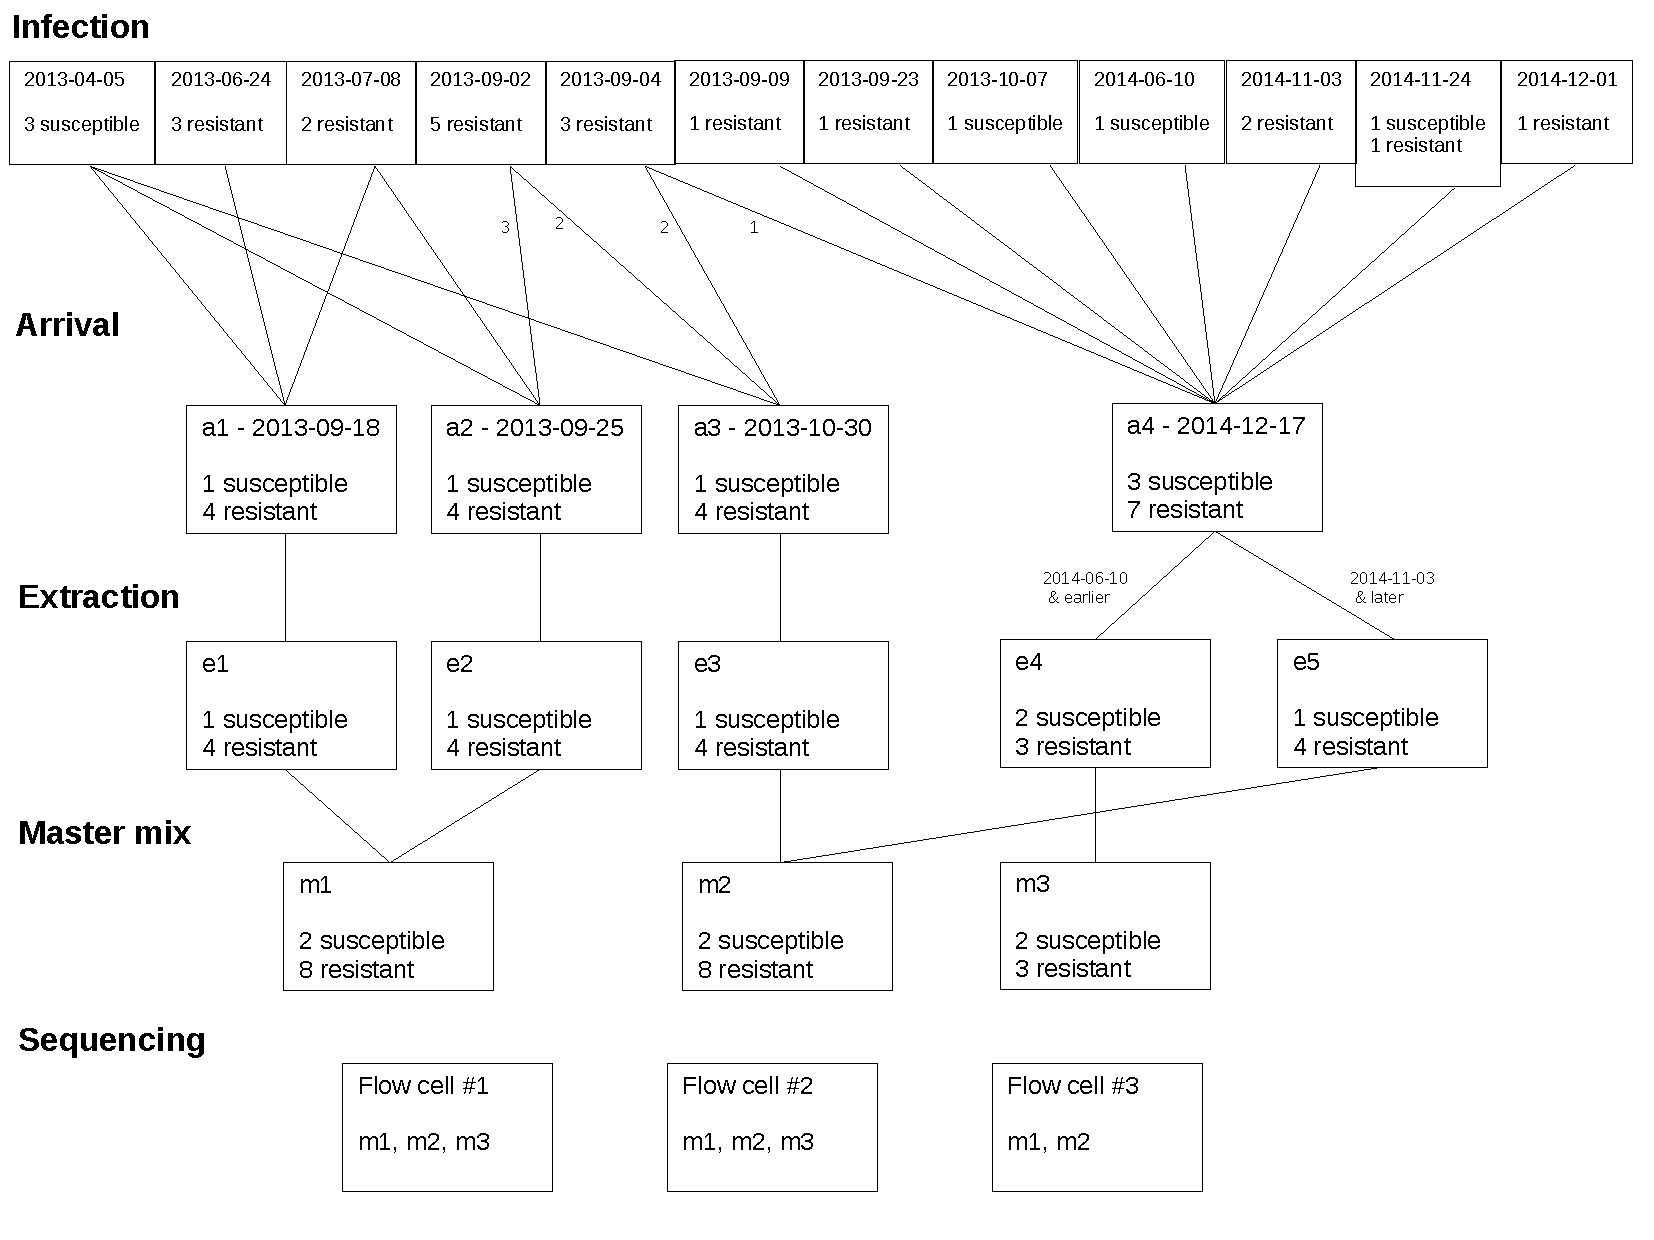
\includegraphics[width=5in]{img/ch03/processing.pdf}
\caption[Batch processing.]{ \textbf{Batch processing.} We designed
  the processing of the samples to minimize the introduction of
  technical batch effects. Specifically, we attempted to balance the
  processing of samples obtained from susceptible and resistant
  individuals. In the diagram, each box represents a
  batch. ``Infection'' labels the batches of the infection
  experiments, ``Arrival'' labels the batch shipments of cell lysates
  arrived in Chicago, USA from Paris, France, ``Extraction'' labels
  the batches of RNA extraction, ``Master Mix'' labels the batches of
  library preparation, and ``Sequencing'' labels the batches of flow
  cells. Each master mix listed in a flow cell batch was sequenced on
  only one lane of that flow cell.  }
\label{fig:process}
\end{figure}


\begin{figure}[!htb]
\centering
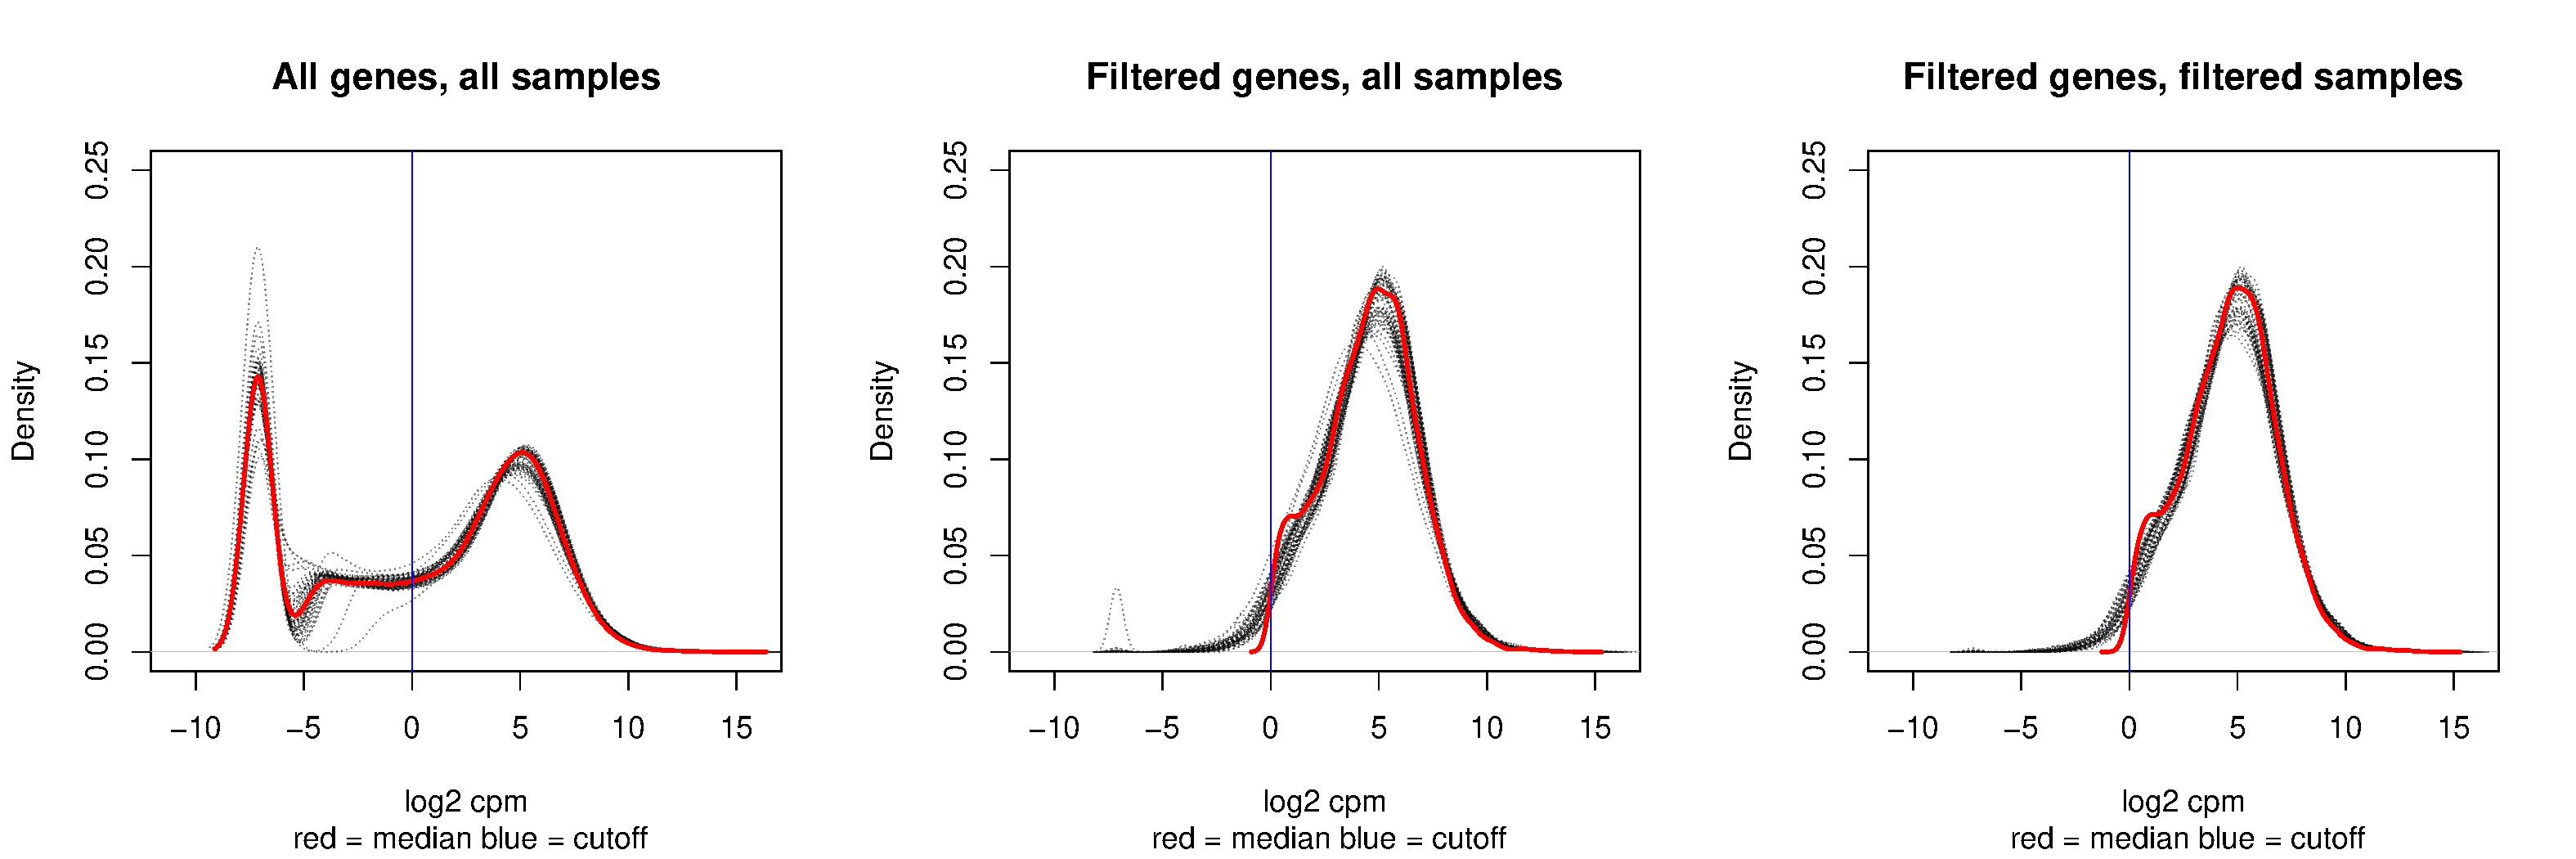
\includegraphics[width=5in]{img/ch03/gene-exp-distribution.pdf}
\caption[Gene expression distributions before and after filtering
  genes and samples.]{ \textbf{Gene expression distributions before
    and after filtering genes and samples.} The log\textsubscript{2}
  counts per million (cpm) of each sample is plotted as a dashed gray
  line. The solid red line represents the median value across all the
  samples. The vertical solid blue line at $x = 0$ represents the
  cutoff used to filter lowly expressed genes based on their median
  log\textsubscript{2} cpm. The left panel is the data from all 19,800
  genes and 50 samples, the middle panel is the data from the 11,336
  genes remaining after removing lowly expressed genes, and the right
  panel is the data from 11,336 genes and the 44 samples remaining
  after removing outliers.  }
\label{fig:gene}
\end{figure}

\begin{figure}[!htb]
\centering
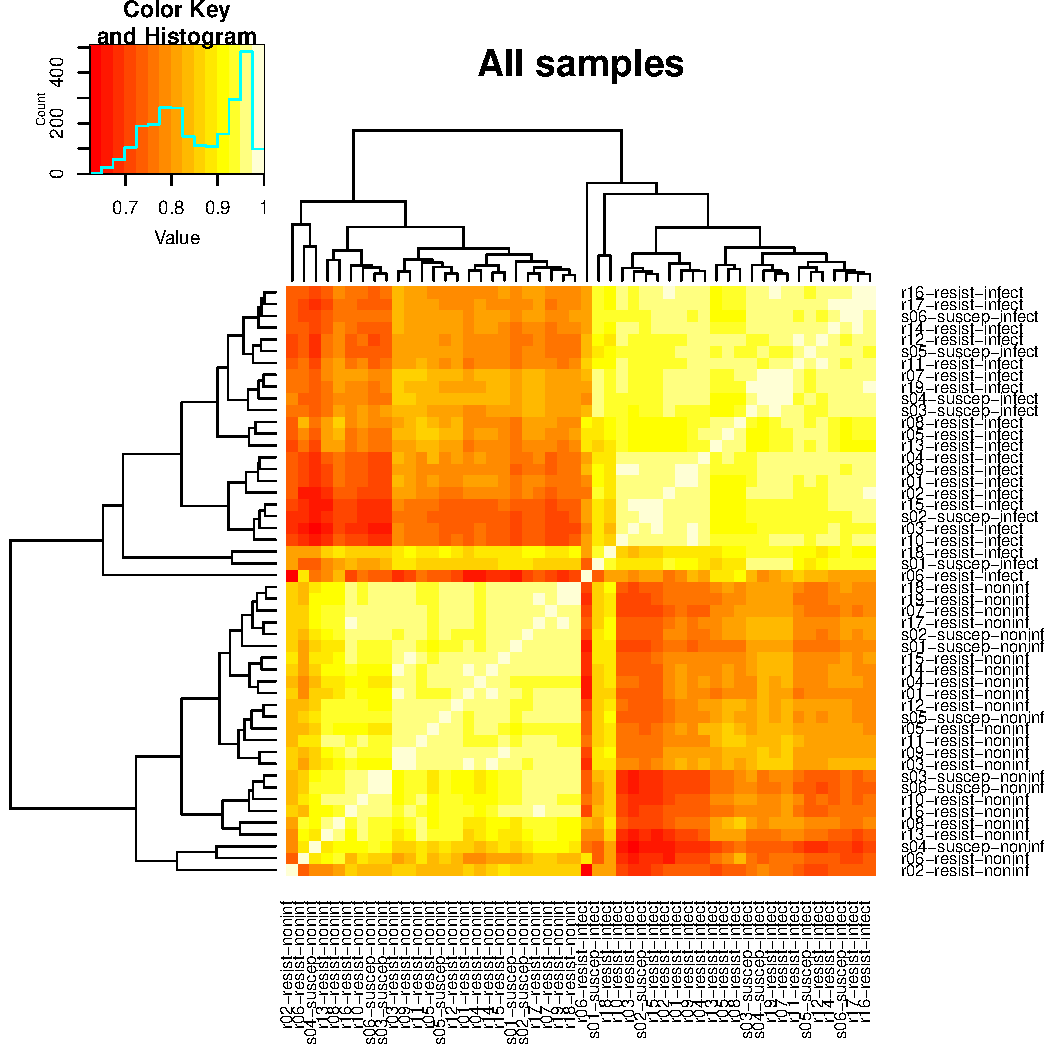
\includegraphics[width=5in]{img/ch03/heatmap-all-samples.pdf}
\caption[Heatmap of correlation matrix of samples.]{ \textbf{Heatmap
    of correlation matrix of samples.} Each square represents the
  Pearson correlation between the log\textsubscript{2} cpm expression
  values of two samples. Red indicates a low correlation of zero and
  white represents a high correlation of 1. The dendrogram displays
  the results of hierarchical clustering with the complete linkage
  method.  The outliers of the non-infected samples are
  s04-suscept-noninf, r02-resist-noninf, and r06-resist-noninf. The
  outliers of the infected samples are s01-suscep-infect,
  r06-resist-infect, and r18-resist-infect.  }
\label{fig:heat-all}
\end{figure}

\begin{figure}[!htb]
\centering
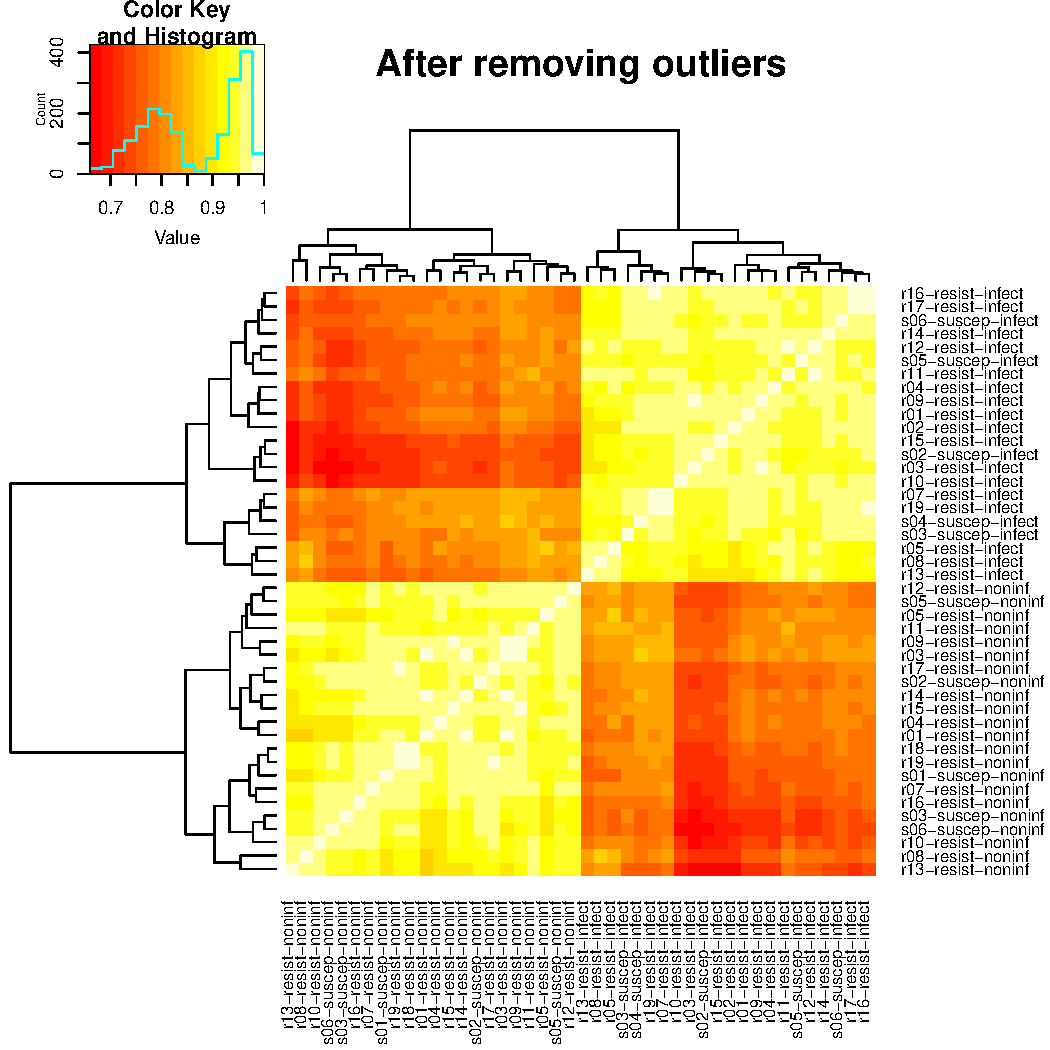
\includegraphics[width=5in]{img/ch03/heatmap-no-outliers.pdf}
\caption[Heatmap of correlation matrix after removing outliers.]{
  \textbf{Heatmap of correlation matrix after removing outliers.} Each
  square represents the Pearson correlation between the
  log\textsubscript{2} cpm expression values of two samples. Red
  indicates a low correlation of zero and white represents a high
  correlation of 1. The dendrogram displays the results of
  hierarchical clustering with the complete linkage method.  }
\label{fig:heat-filt}
\end{figure}


\begin{figure}[!htb]
\centering 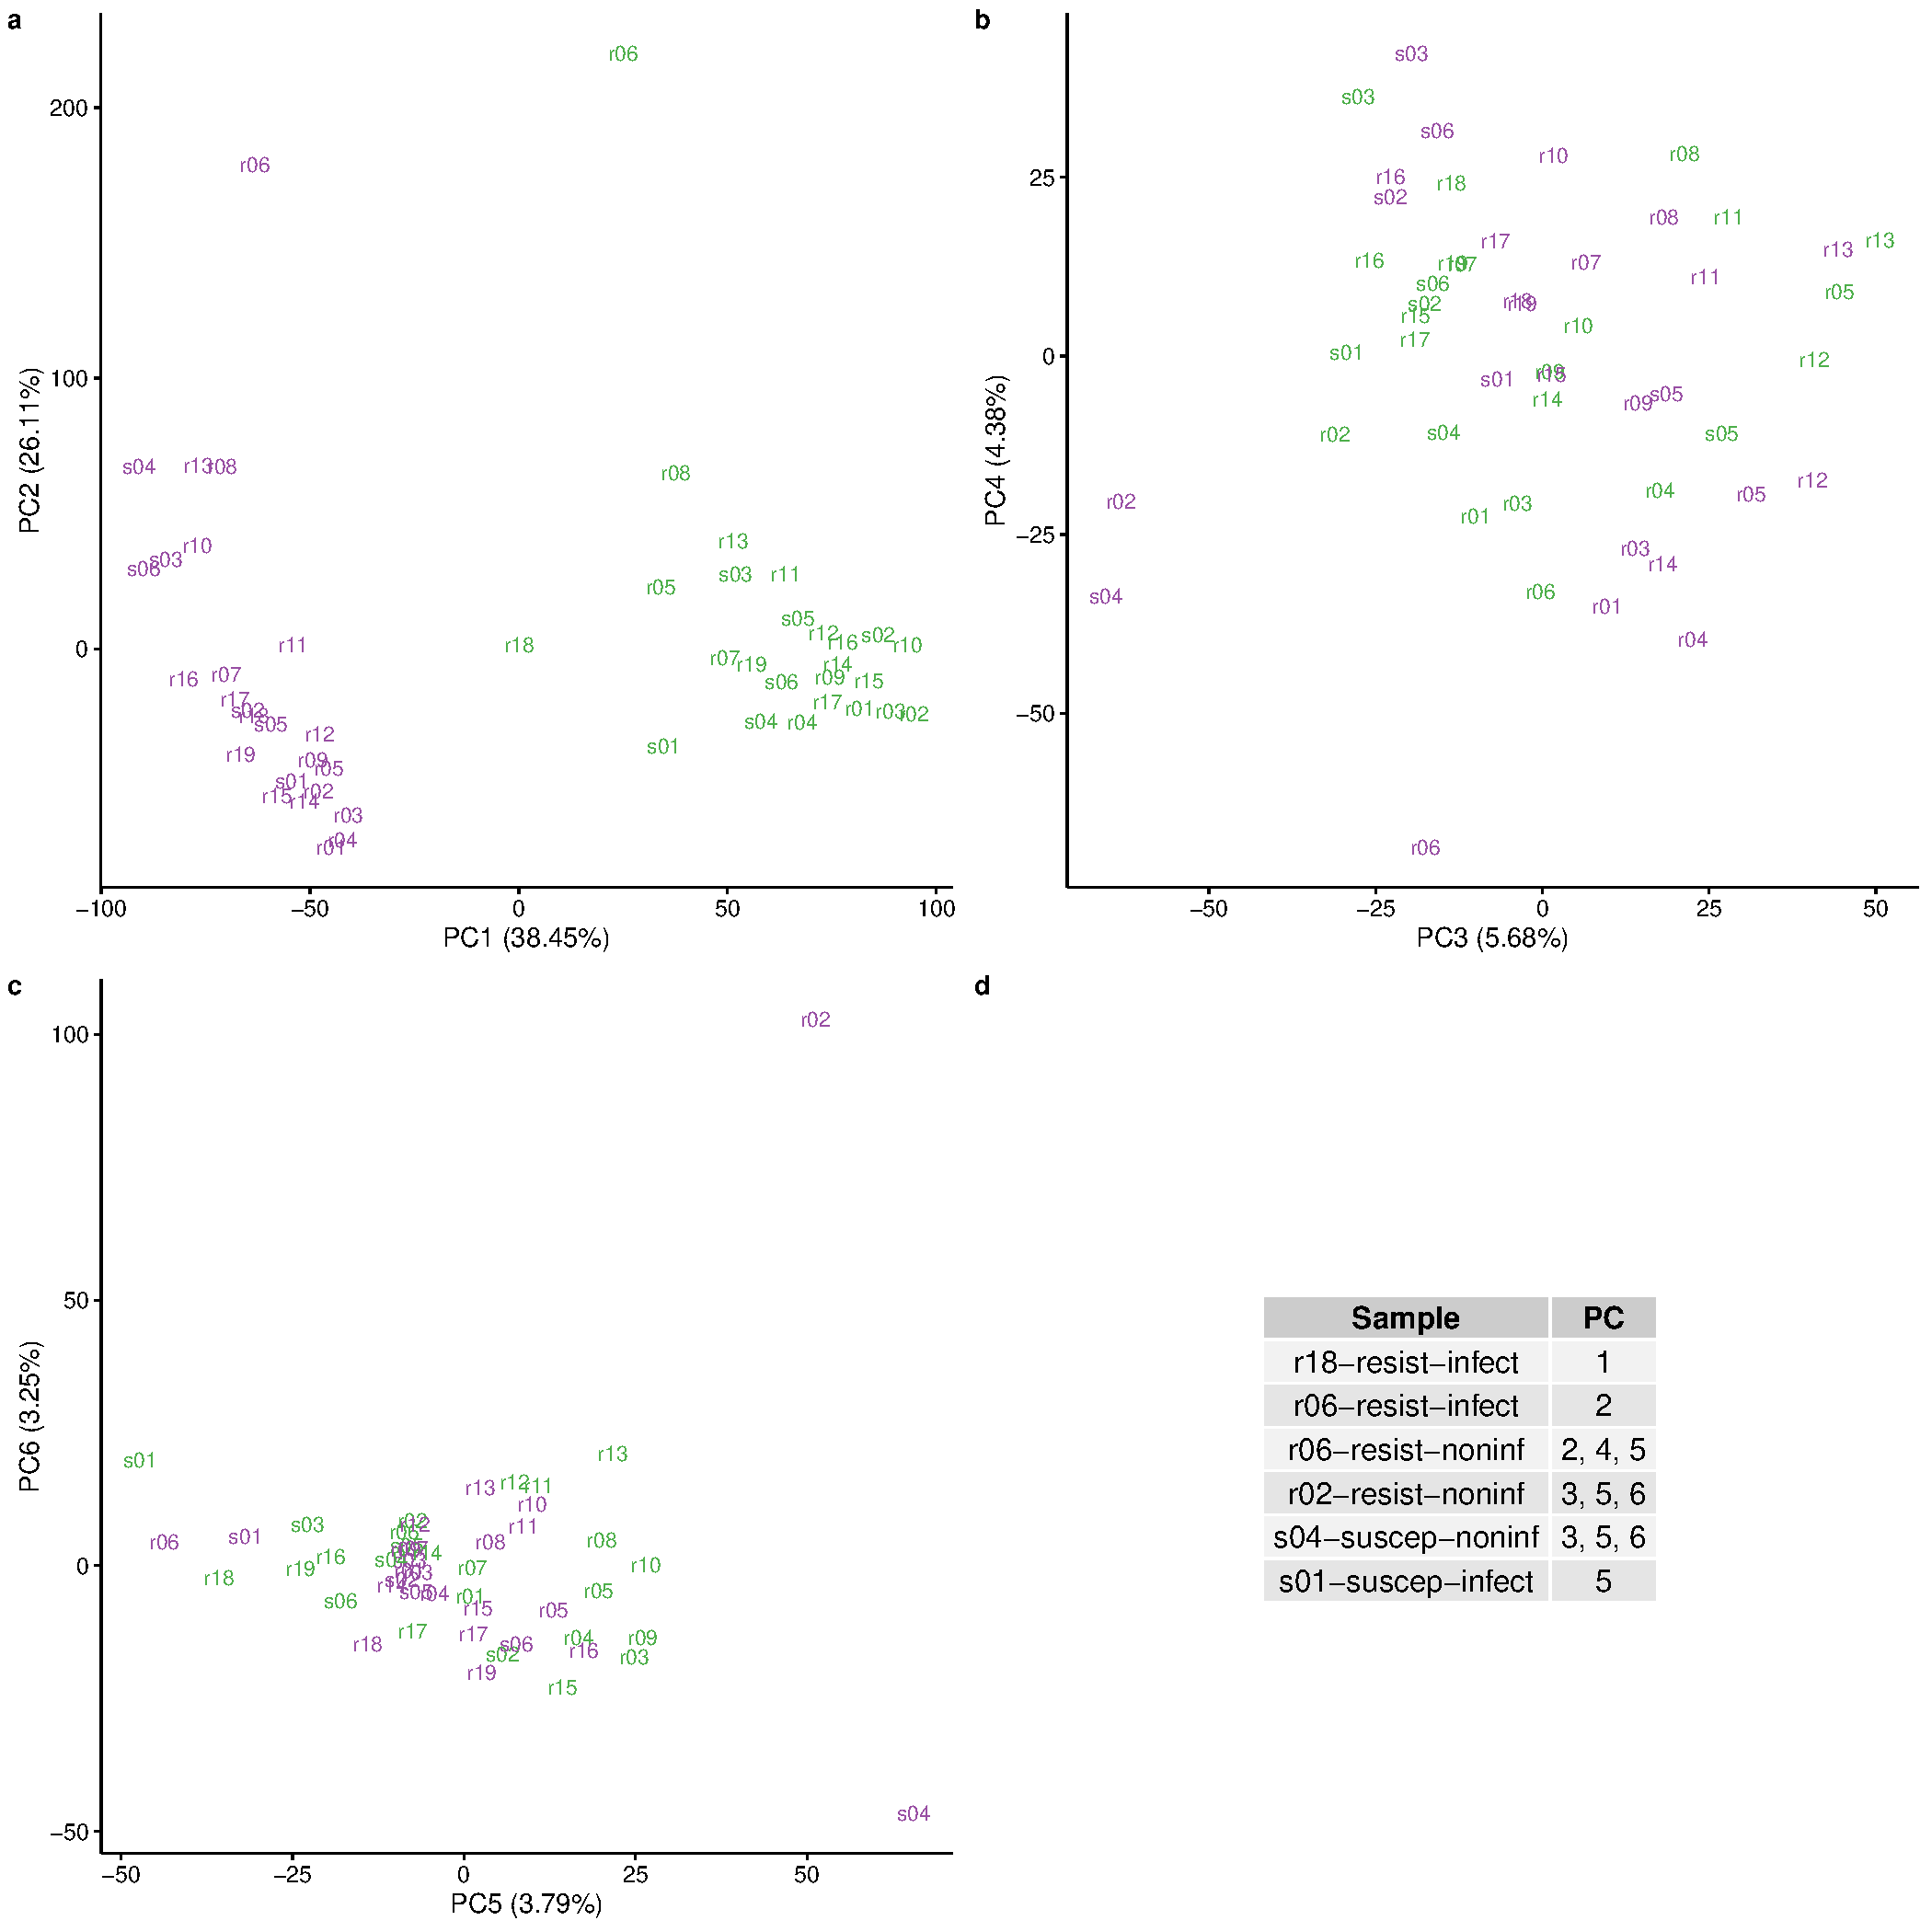
\includegraphics[width=5in]{img/ch03/outliers.pdf}
\caption[Principal components analysis (PCA) to identify outliers.]{
  \textbf{Principal components analysis (PCA) to identify outliers.}
  PC1 versus PC2 (a), PC3 versus PC4 (b), and PC5 versus PC6 (c). Each
  sample is represented by its 3-letter ID. ``s'' stands for
  susceptible and ``r'' for resistant, and the text is colored on the
  basis of treatment status (purple is non-infected; green is
  infected). The value is parentheses in each axis is the percentage
  of total variation accounted for by that PC. The outliers are listed
  in (d). These samples do not fall within 2 standard deviations of
  the mean value of the PCs listed in the right column. Note that a
  separate mean was calculated for the non-infected and infected
  samples for PC1 only.  }
\label{fig:outliers}
\end{figure}


\begin{figure}[!htb]
\centering 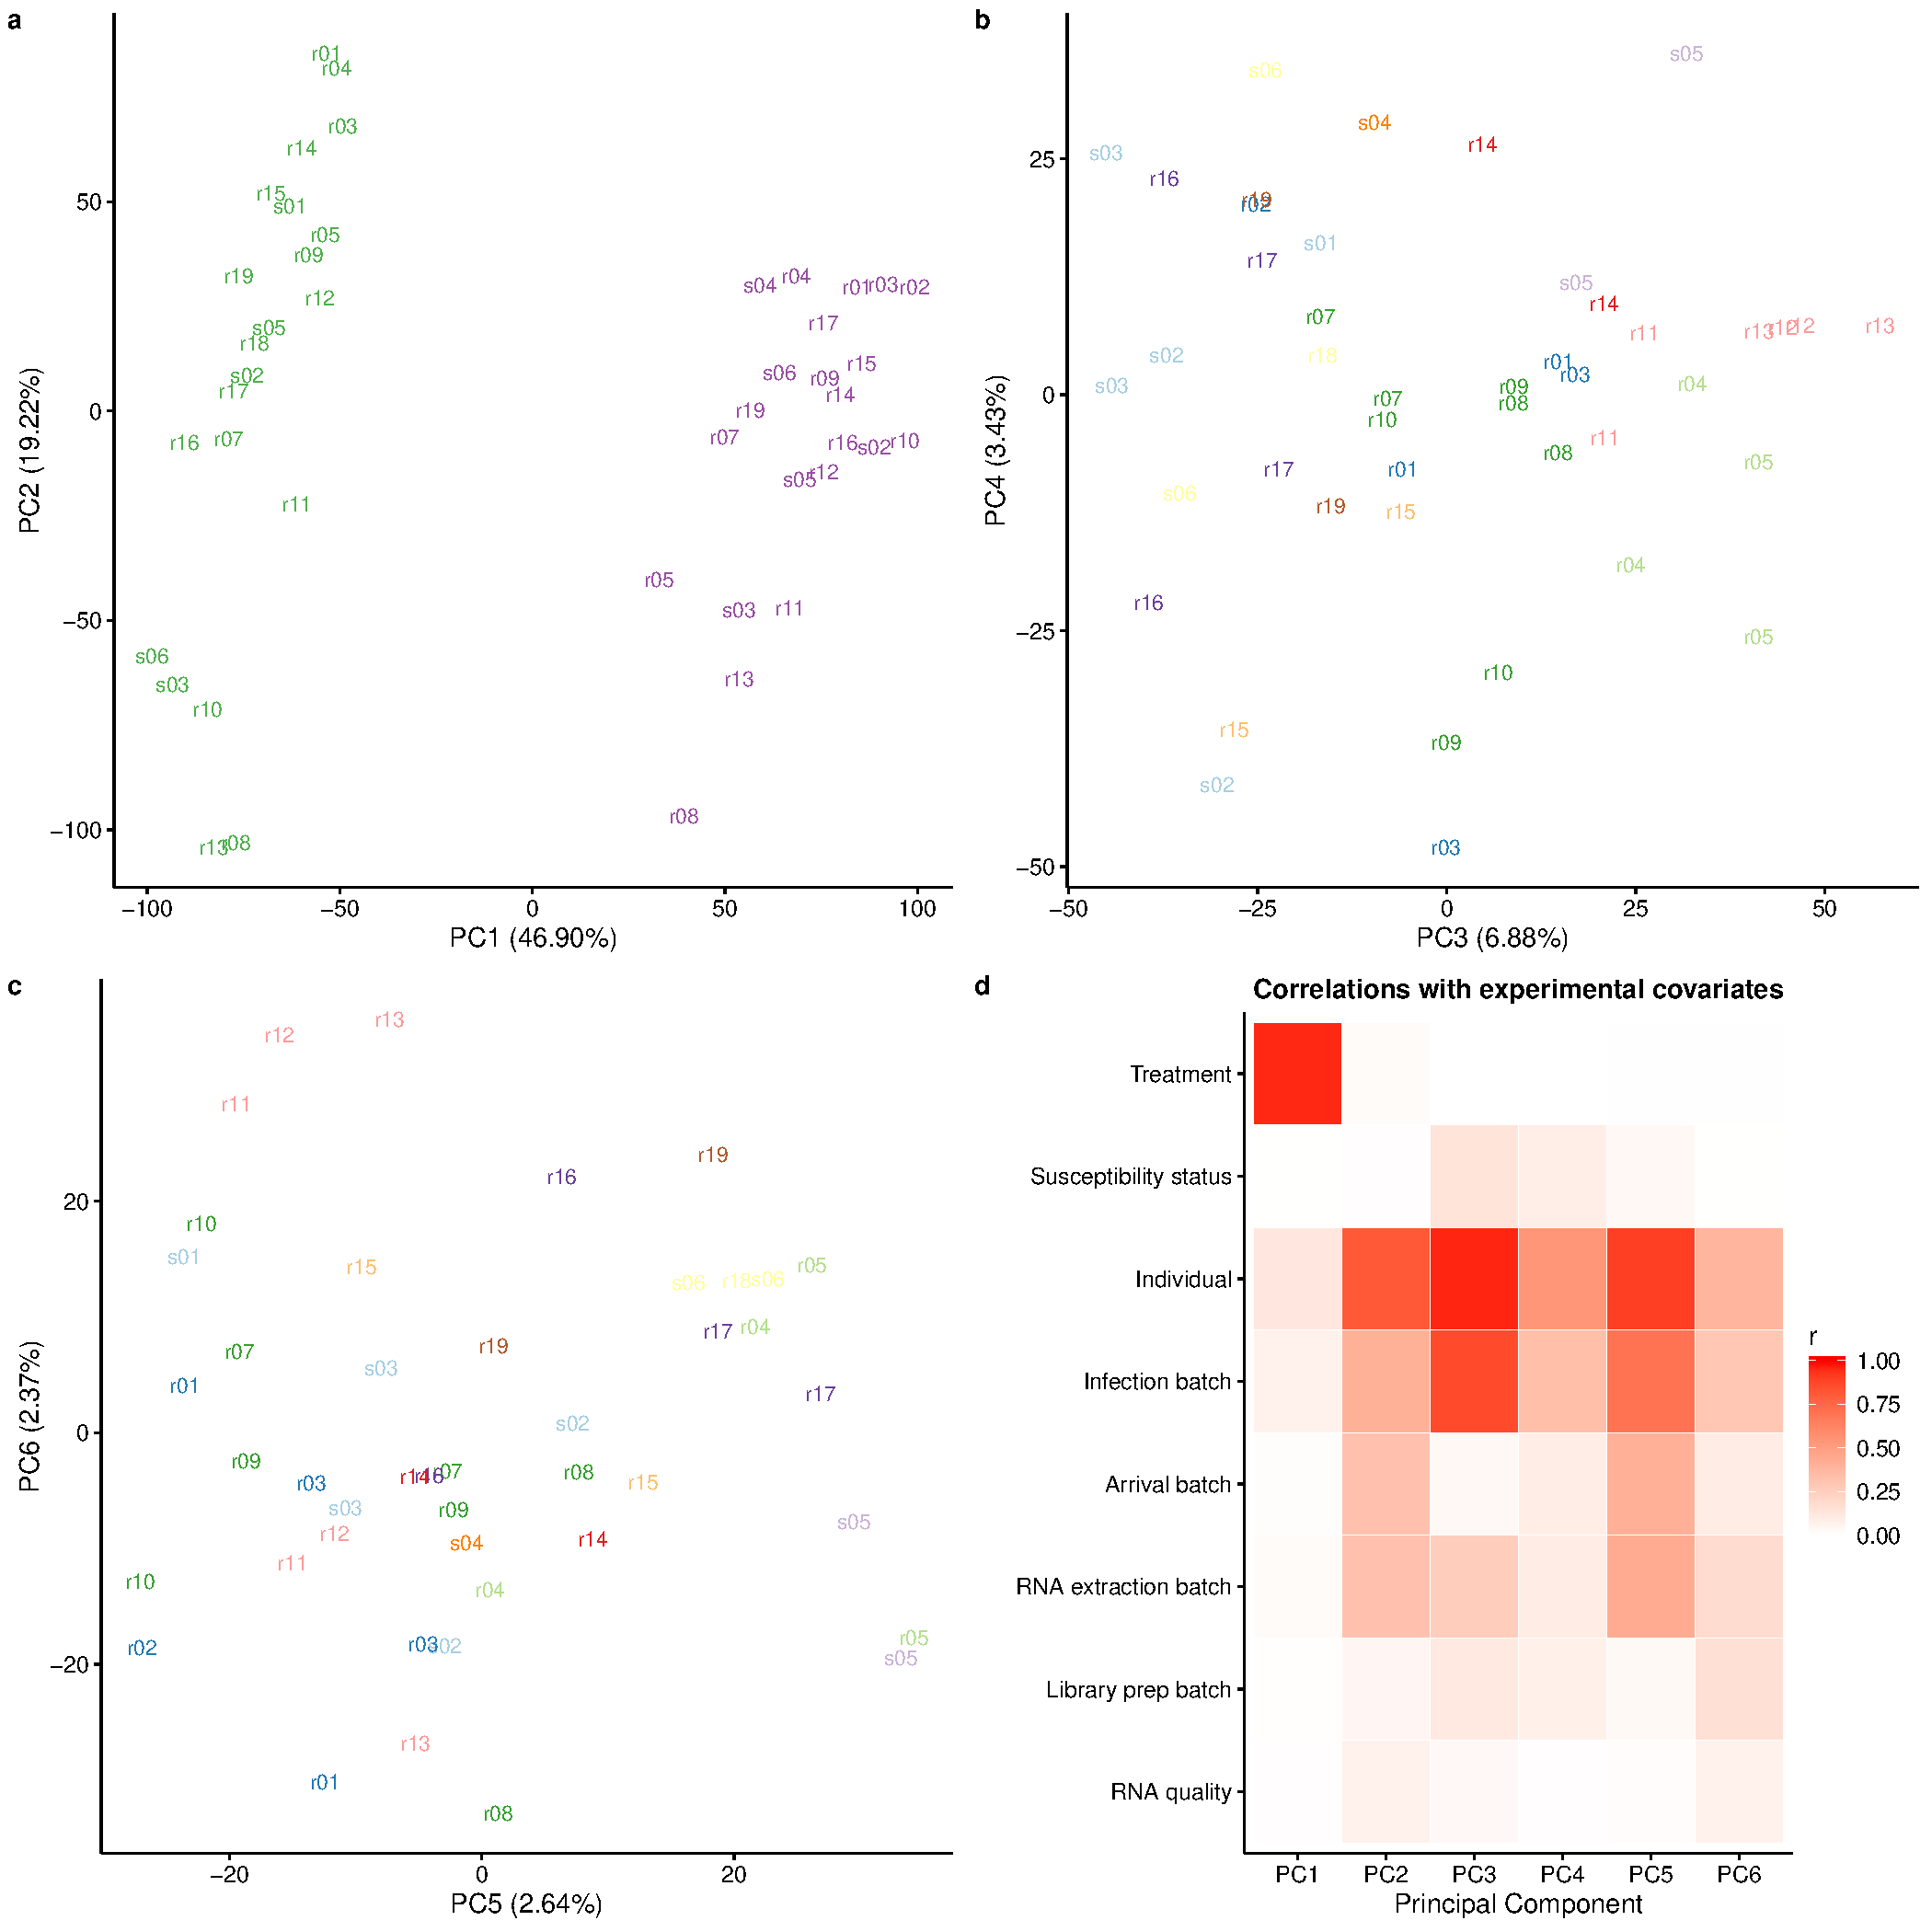
\includegraphics[width=5in]{img/ch03/batch-pca.pdf}
\caption[Check for technical batch effects using principal components
  analysis (PCA).]{ \textbf{Check for technical batch effects using
    principal components analysis (PCA).} (a) PC1 versus PC2. The text
  labels are the individual identifiers. Purple indicates non-infected
  samples and green indicates infected. (b) PC3 versus PC4. The colors
  indicate the different infection batches. (c) PC5 versus PC6. The
  colors indicate the different infection batches. (d) The Pearson
  correlation of PCs 1-6 with each of the recorded biological and
  technical covariates. The correlations vary from 0 (white) to 1
  (red).  }
\label{fig:batch-effect}
\end{figure}

\begin{figure}[!htb]
\centering 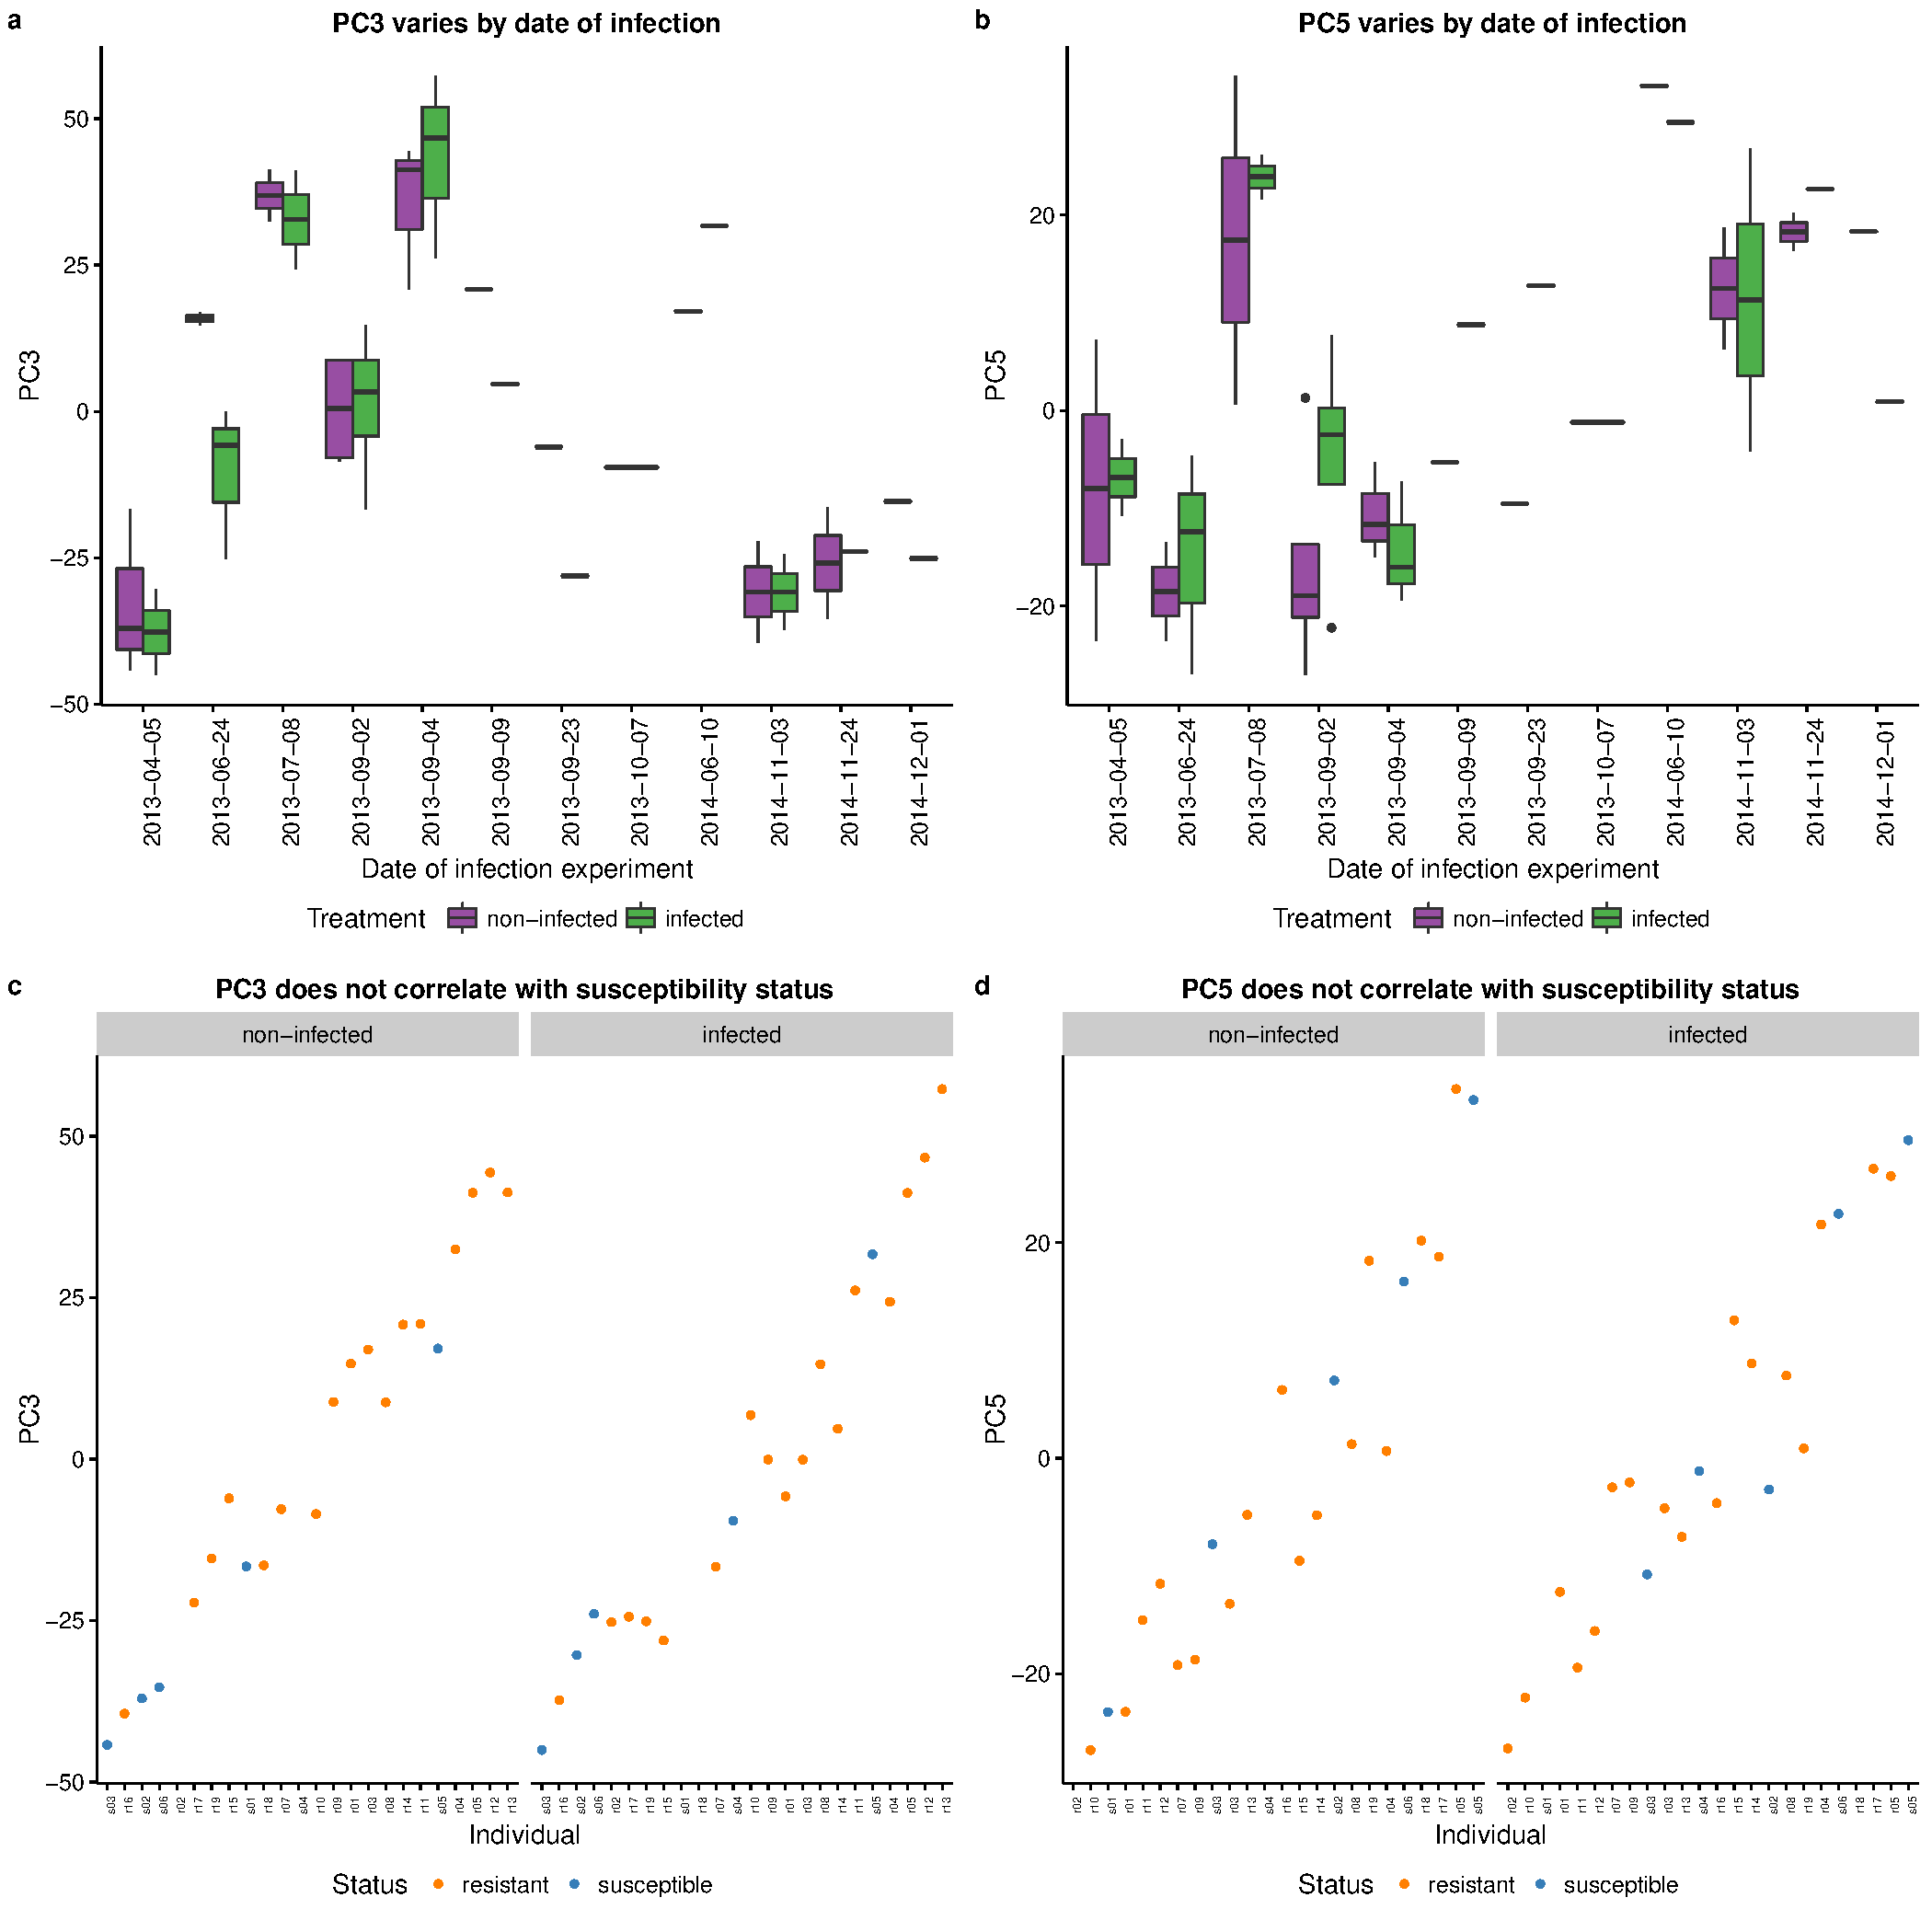
\includegraphics[width=5in]{img/ch03/batch-infection.pdf}
\caption[Check for confounding effect of infection batch.]{
  \textbf{Check for confounding effect of infection batch.} PC3 (a)
  and PC5 (b) varied by the date of infection. Non-infected samples
  are in purple and infected samples in green. Importantly, however,
  this technical variation arising from infection batch did not
  correlate with the susceptibility status of the individuals (c and
  d). Resistant individuals are in orange and susceptible individuals
  in blue.  }
\label{fig:infection}
\end{figure}

\begin{figure}[!htb]
\centering 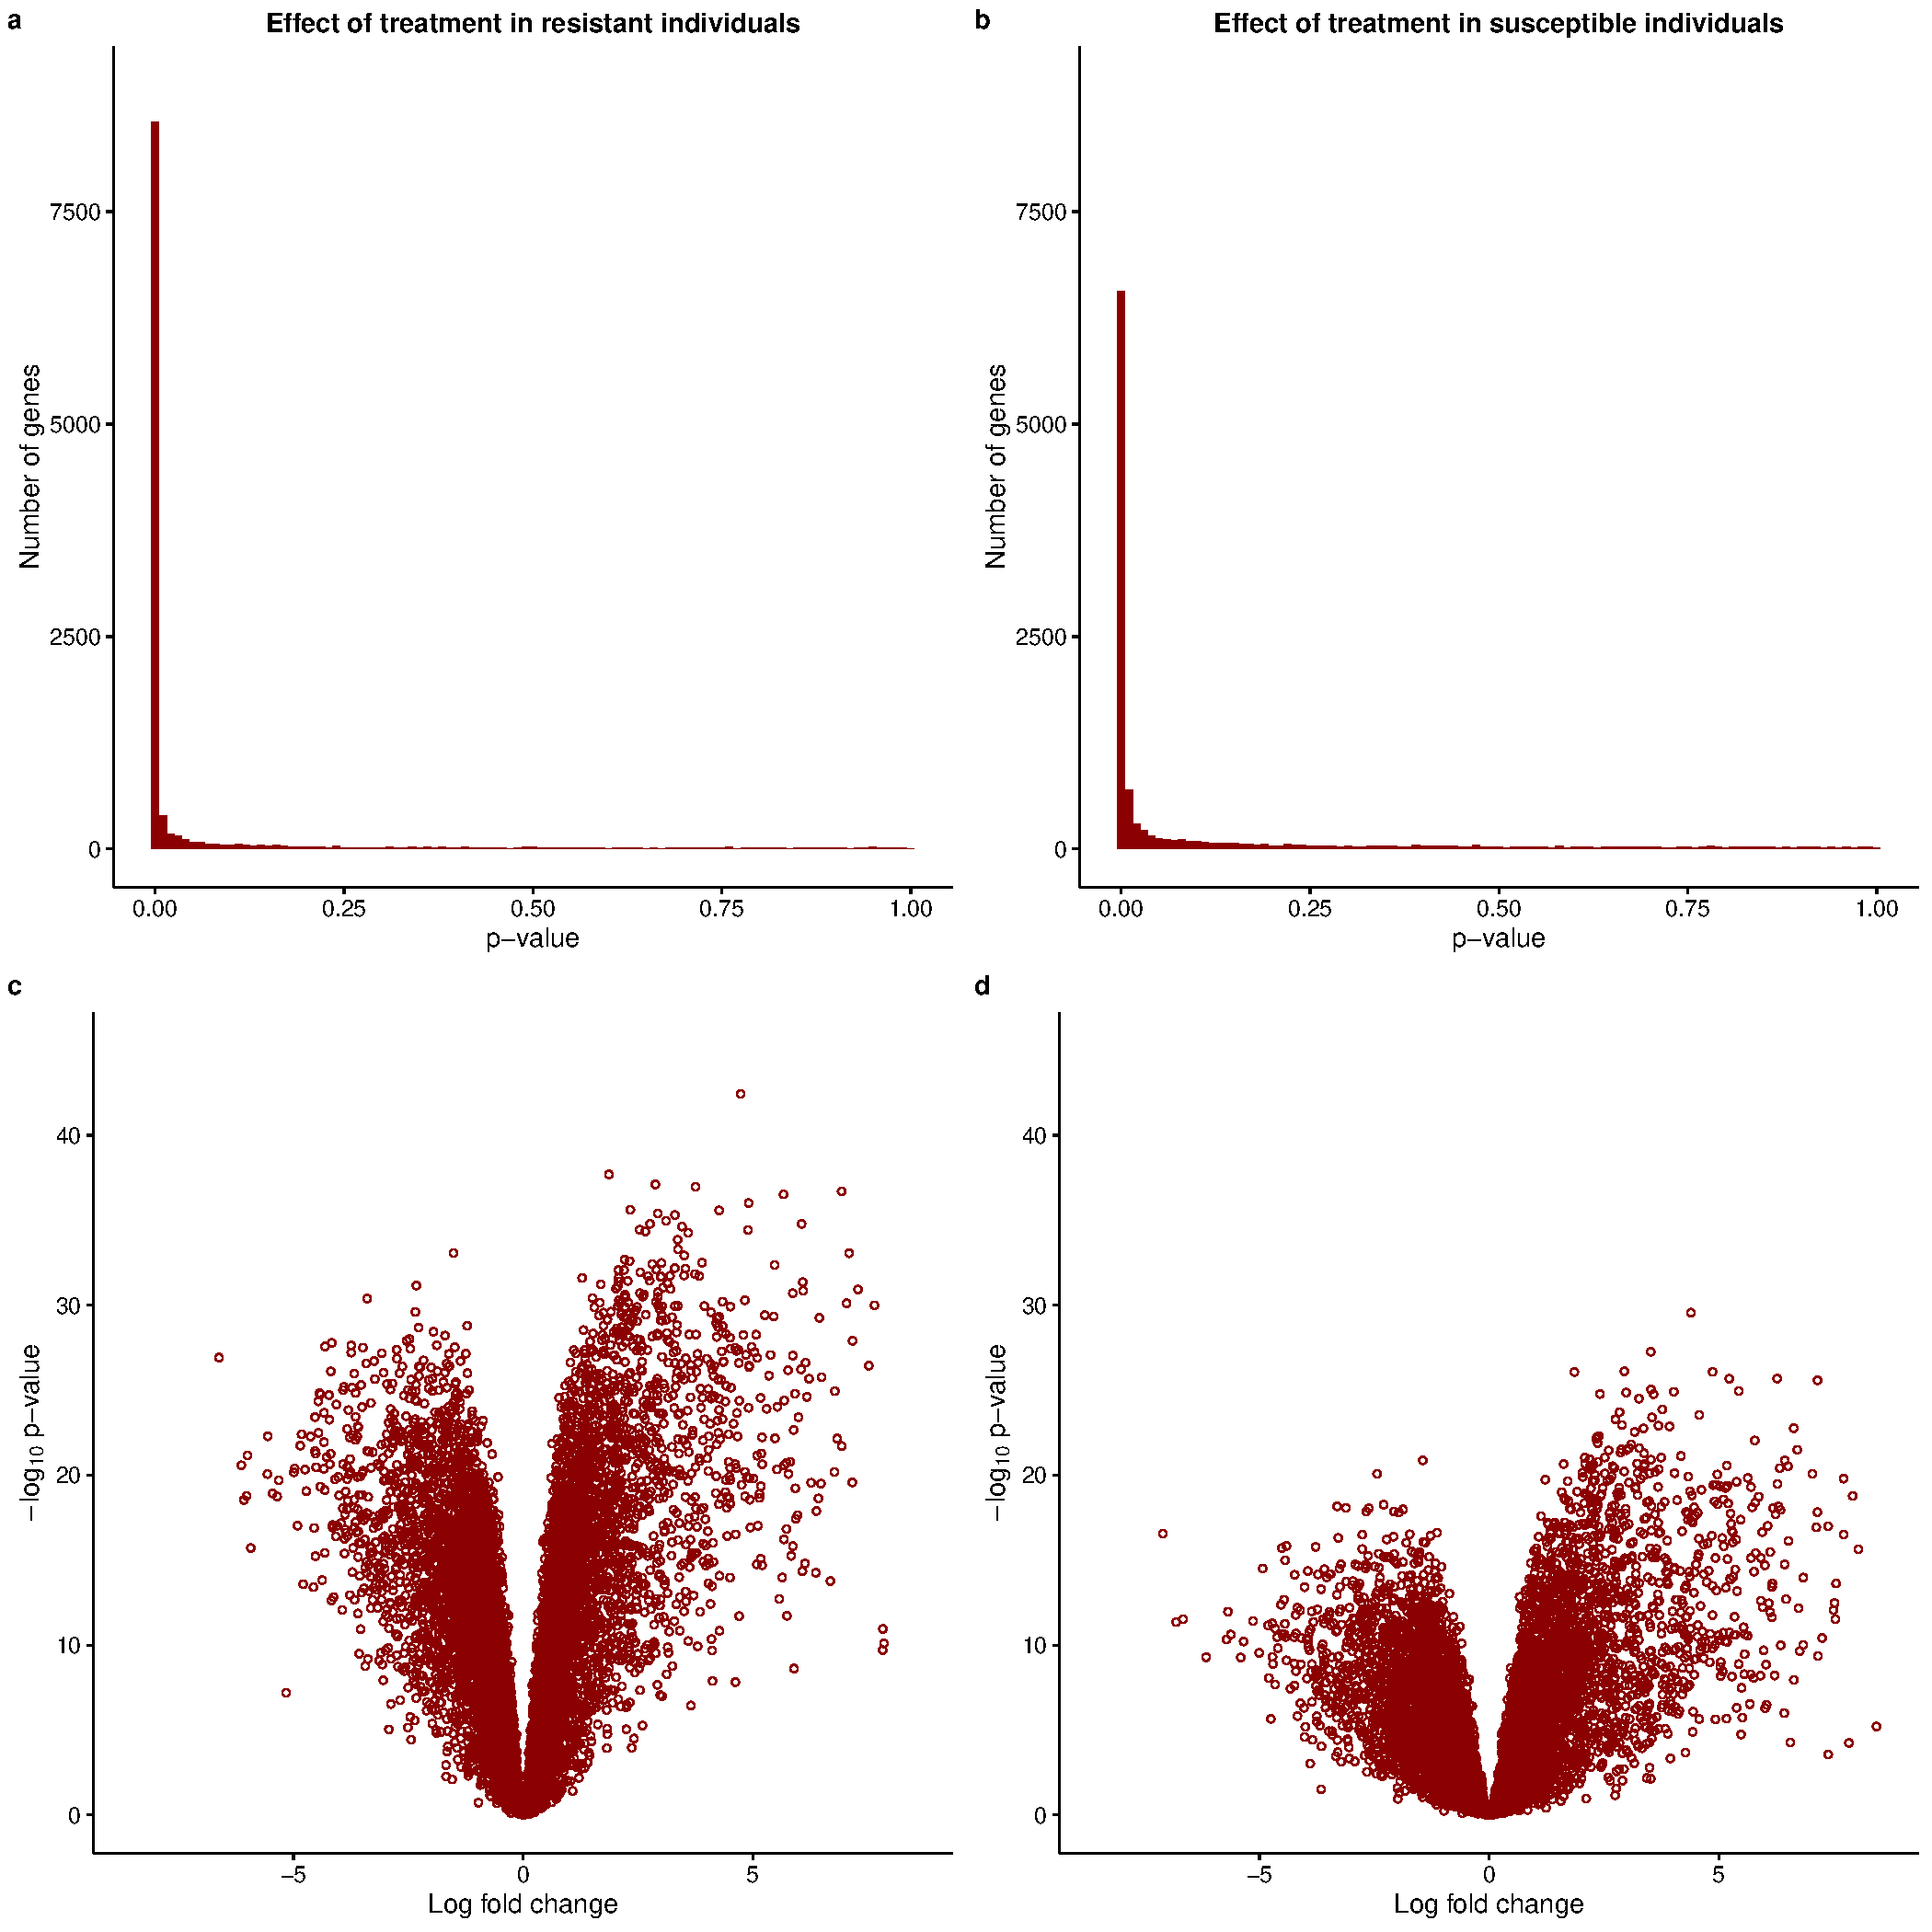
\includegraphics[width=5in]{img/ch03/limma-supp.pdf}
\caption[Effect of treatment with MTB.]{ \textbf{Effect of treatment
    with MTB.} The top panel contains the distribution of unadjusted
  p-values after testing for differential expression between the
  non-infected and infected states in (a) resistant and (b)
  susceptible individuals. The bottom panel contains the corresponding
  volcano plots for the (c) resistant and (d) susceptible individuals.
  The x-axis is the log fold change in gene expression level between
  susceptible and resistant individuals and the y-axis is the
  –log\textsubscript{10} p-value. Red indicates genes which are
  significant differentially expressed with a q-value less than 10\%.
  Because of the extremely skewed p-value distribution, all genes are
  significantly differentially expressed at this false discovery rate.
}
\label{fig:limma-supp}
\end{figure}

\begin{figure}[!htb]
\centering 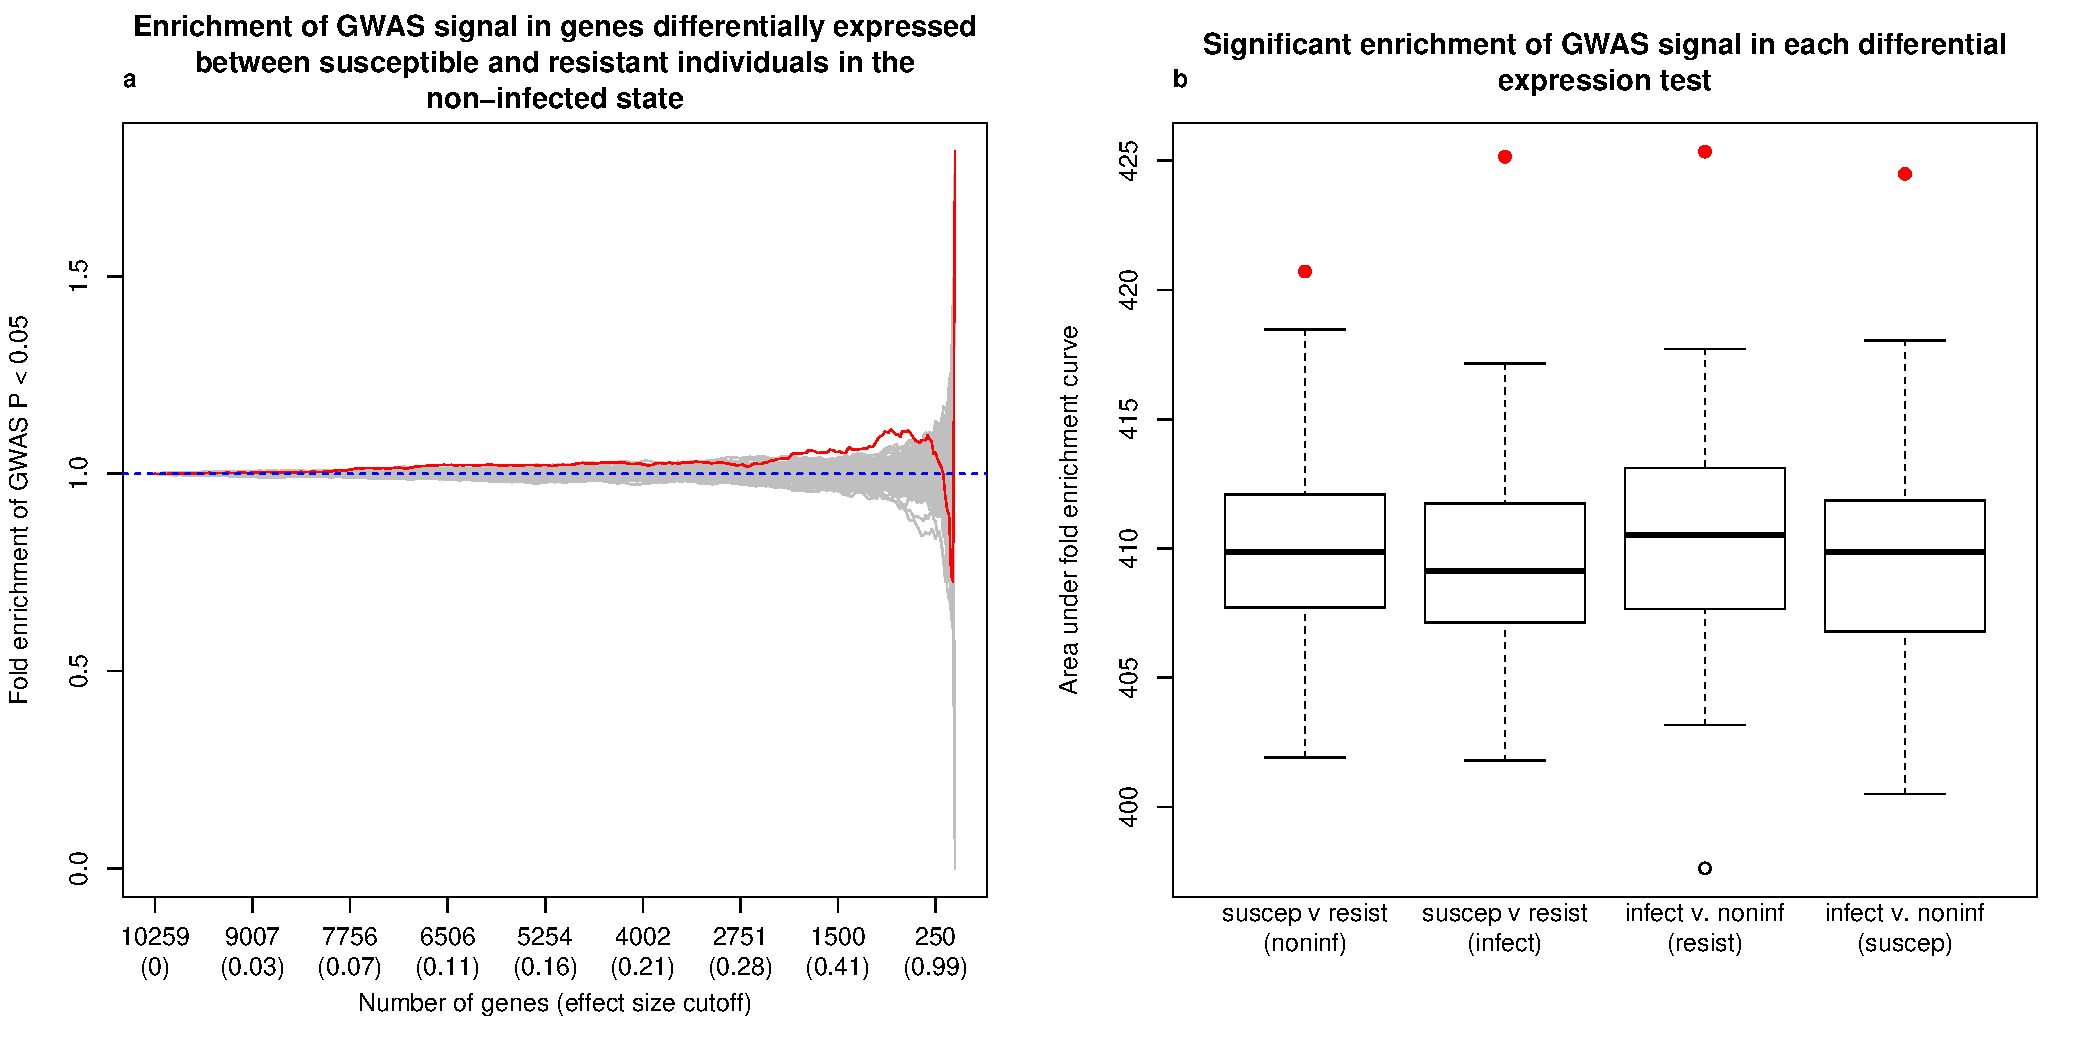
\includegraphics[width=5in]{img/ch03/gwas-supp.pdf}
\caption[Comparison of differential expression and Ghana GWAS
  results.]{ \textbf{Comparison of differential expression and Ghana
    GWAS results.} (a) The y-axis is the fold enrichment (y-axis) of
  genes assigned a SNP with p-value less than 0.05 from the GWAS in
  Ghana \citep{Thye2010}. The x-axis is bins of genes with
  increasingly stringent effect size cutoffs of the absolute log fold
  change between susceptible and resistant individuals in the
  non-infected state. The effect size cutoffs were chosen such that
  each bin from left to right contained approximately 25 fewer
  genes. The red line is the results from the actual data. The grey
  lines are the results from 100 permutations. The dashed blue line at
  y=1 is the null expectation. (b) The x-axis is each of the 4
  differential expression tests performed. The y-axis is the area
  under the curve of the fold enrichment. The boxplot is the result of
  the 100 permutations, and the red point is the result from the
  actual data. As a reference, the leftmost boxplot corresponds to the
  enrichment plot in (a).  }
\label{fig:gwas-supp}
\end{figure}

\begin{figure}[!htb]
\centering
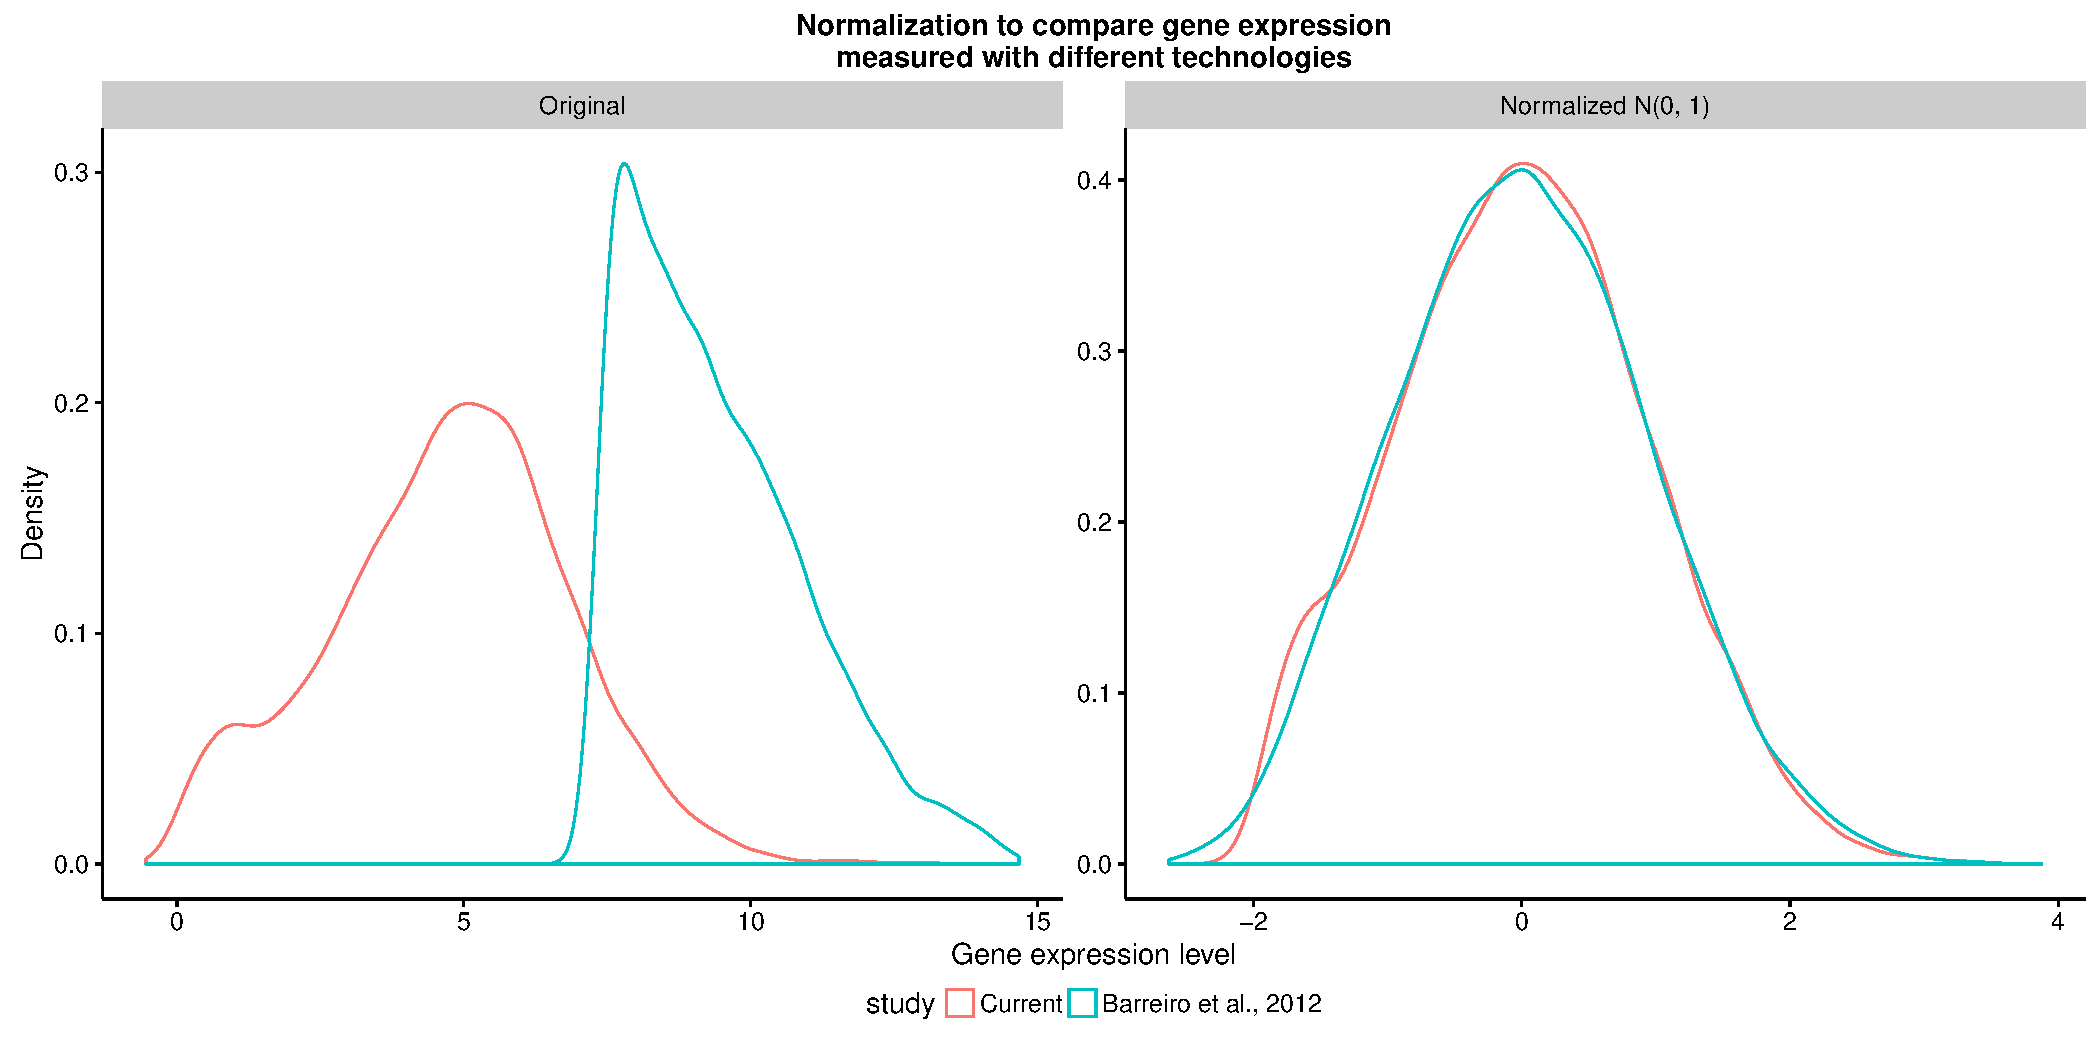
\includegraphics[width=5in]{img/ch03/combined-distributions.pdf}
\caption[Normalizing gene expression distributions.]{
  \textbf{Normalizing gene expression distributions.} (left) The
  distribution of the median log2 cpm of the RNA-seq data from the
  current study in red compared to the distribution of the median gene
  expression levels of the microarray data from Barreiro et al., 2012
  \citep{Barreiro2012} in blue. (right) The distributions of the same
  data sets after normalizing each sample to a standard normal
  distribution.  }
\label{fig:combined-dist}
\end{figure}

\begin{figure}[!htb]
\centering 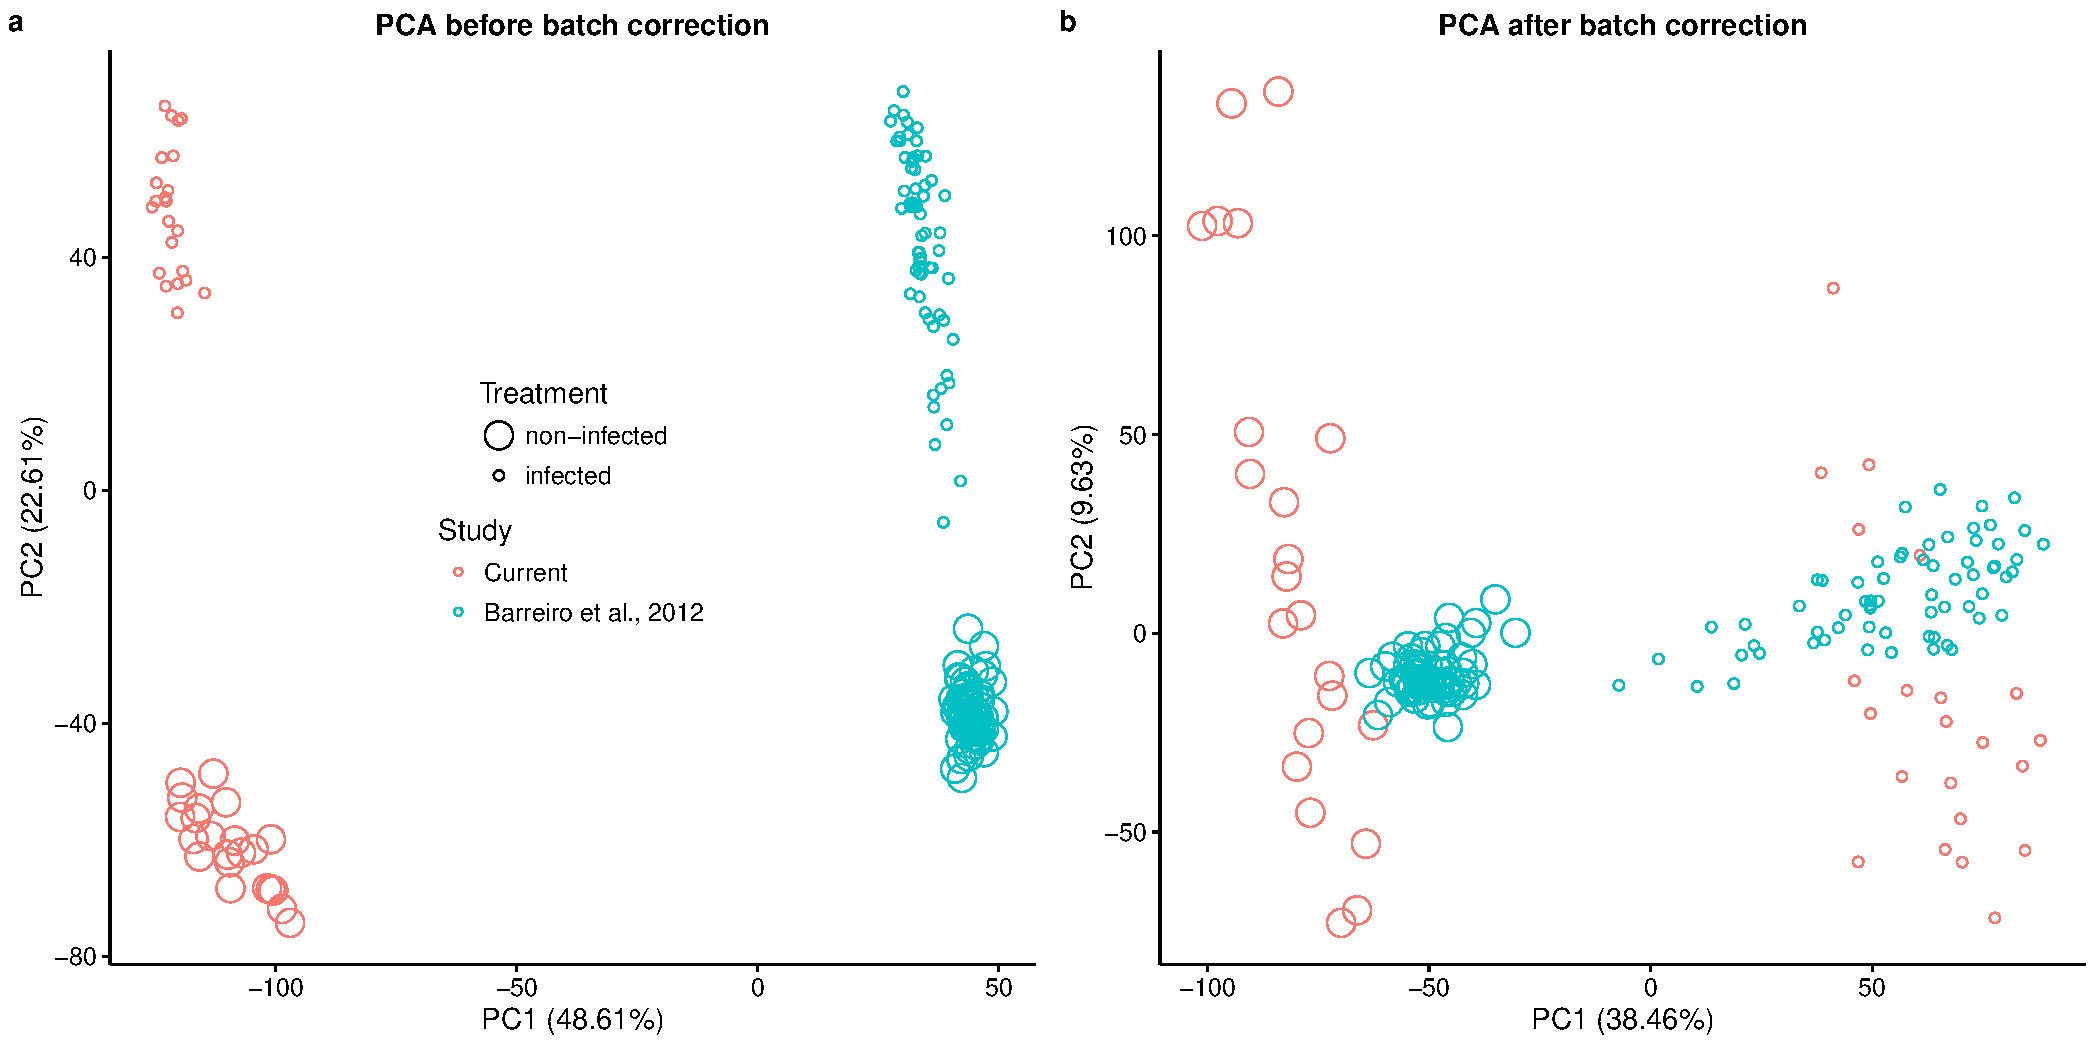
\includegraphics[width=5in]{img/ch03/combined-pca.pdf}
\caption[Principal components analysis (PCA) of combined data sets.]{
  \textbf{Principal components analysis (PCA) of combined data sets.}
  (a) PC1 versus PC2 of the combined data set of the RNA-seq data from
  the current study (red) and the microarray data from Barreiro et
  al., 2012 \citep{Barreiro2012} (blue). The large circles are
  non-infected samples, and the small circles are infected
  samples. The value in parentheses is the percentage of the total
  variation accounted for by that PC. (b) The same data after
  regressing the original PC1 in (a).  }
\label{fig:combined-pca}
\end{figure}

\begin{figure}[!htb]
\centering
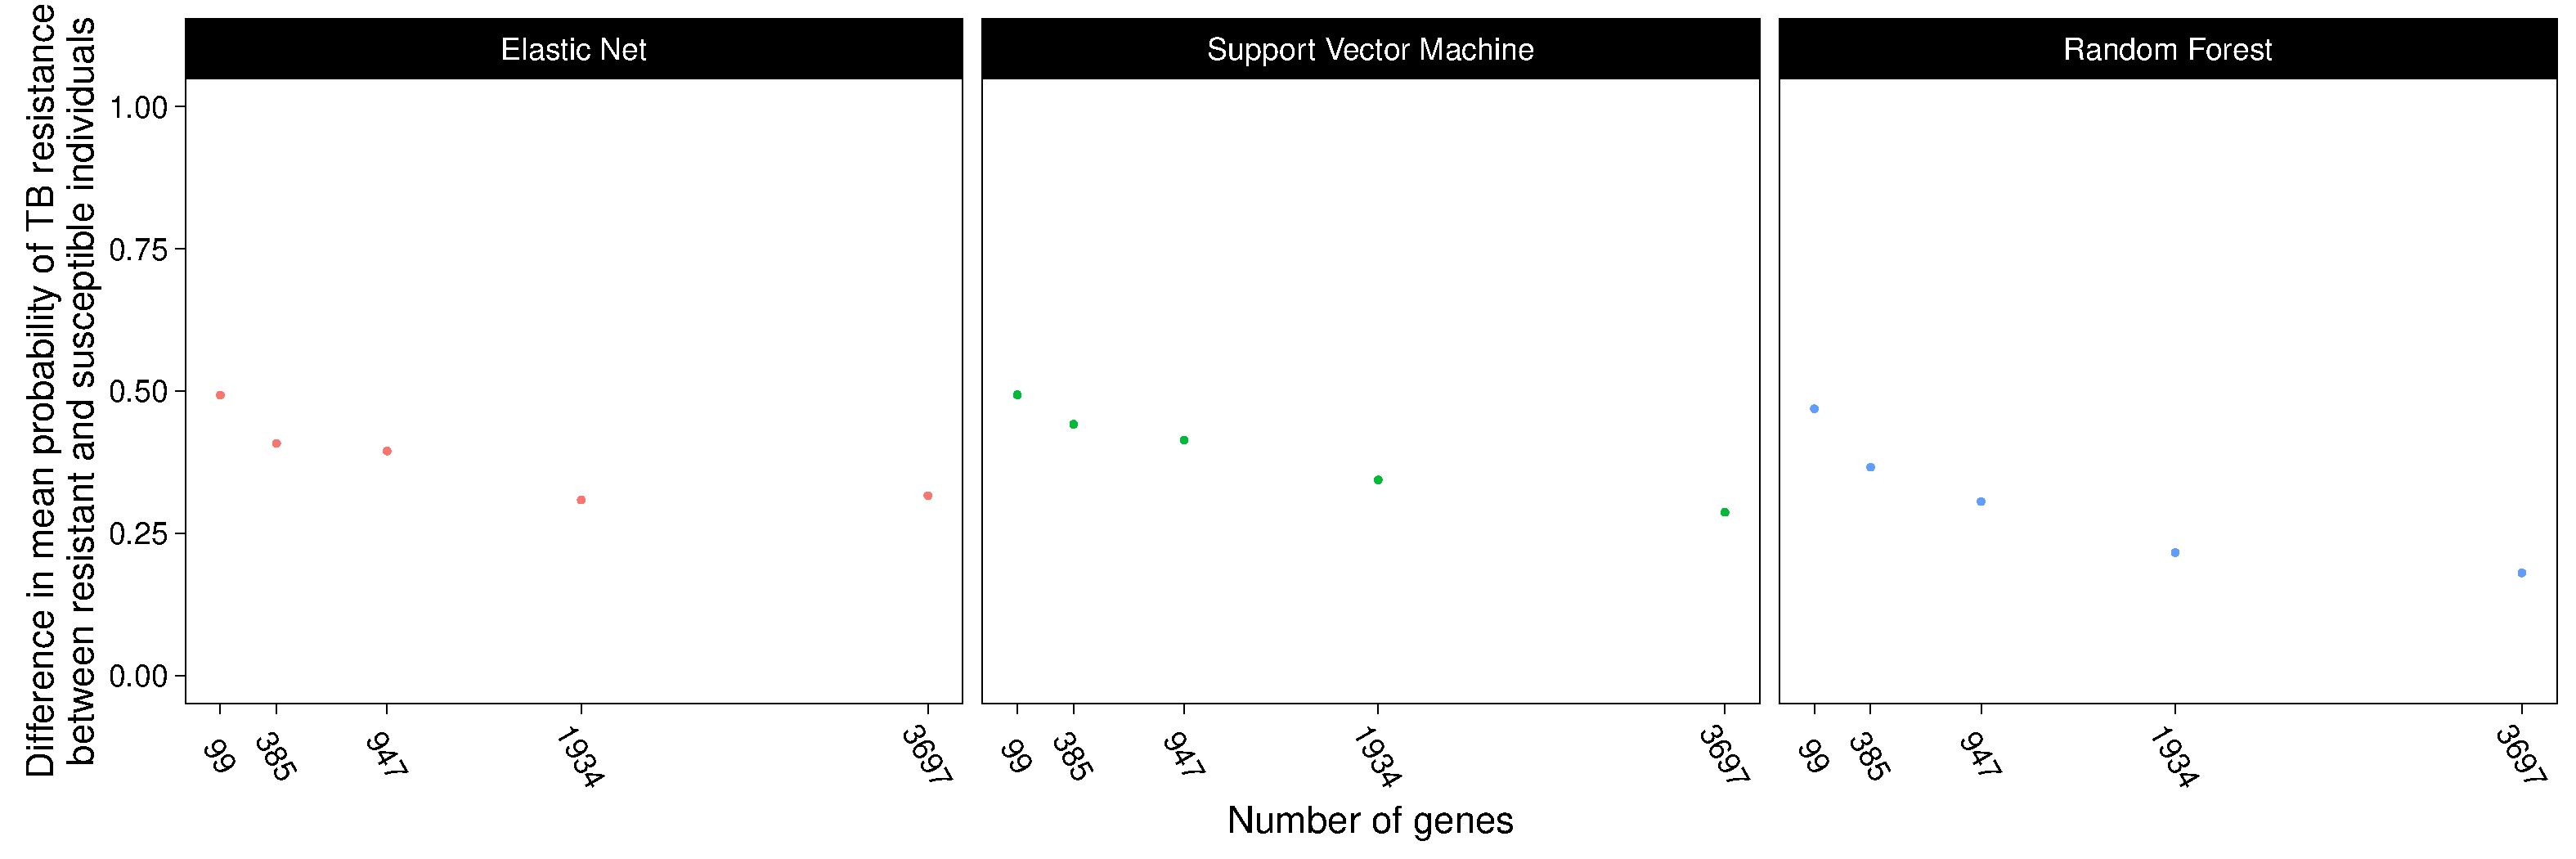
\includegraphics[width=5in]{img/ch03/classifier-compare.pdf}
\caption[Comparing the classification results of different methods and
  number of input genes.]{ \textbf{Comparing the classification
    results of different methods and number of input genes.} We
  compared 3 different machine learning methods (elastic net, support
  vector machine, random forest) and used 5 different sets of input
  genes. The input genes (x-axis) were obtained by varying the q-value
  cutoff for differential expression between susceptible and resistant
  individuals in the non-infected state from 5\% to 25\%. The
  evaluation metric (y-axis) was the difference of the mean assigned
  probability of being TB resistant between the known resistant and
  susceptible individuals in the current study.  }
\label{fig:class-compare}
\end{figure}

\begin{figure}[!htb]
\centering 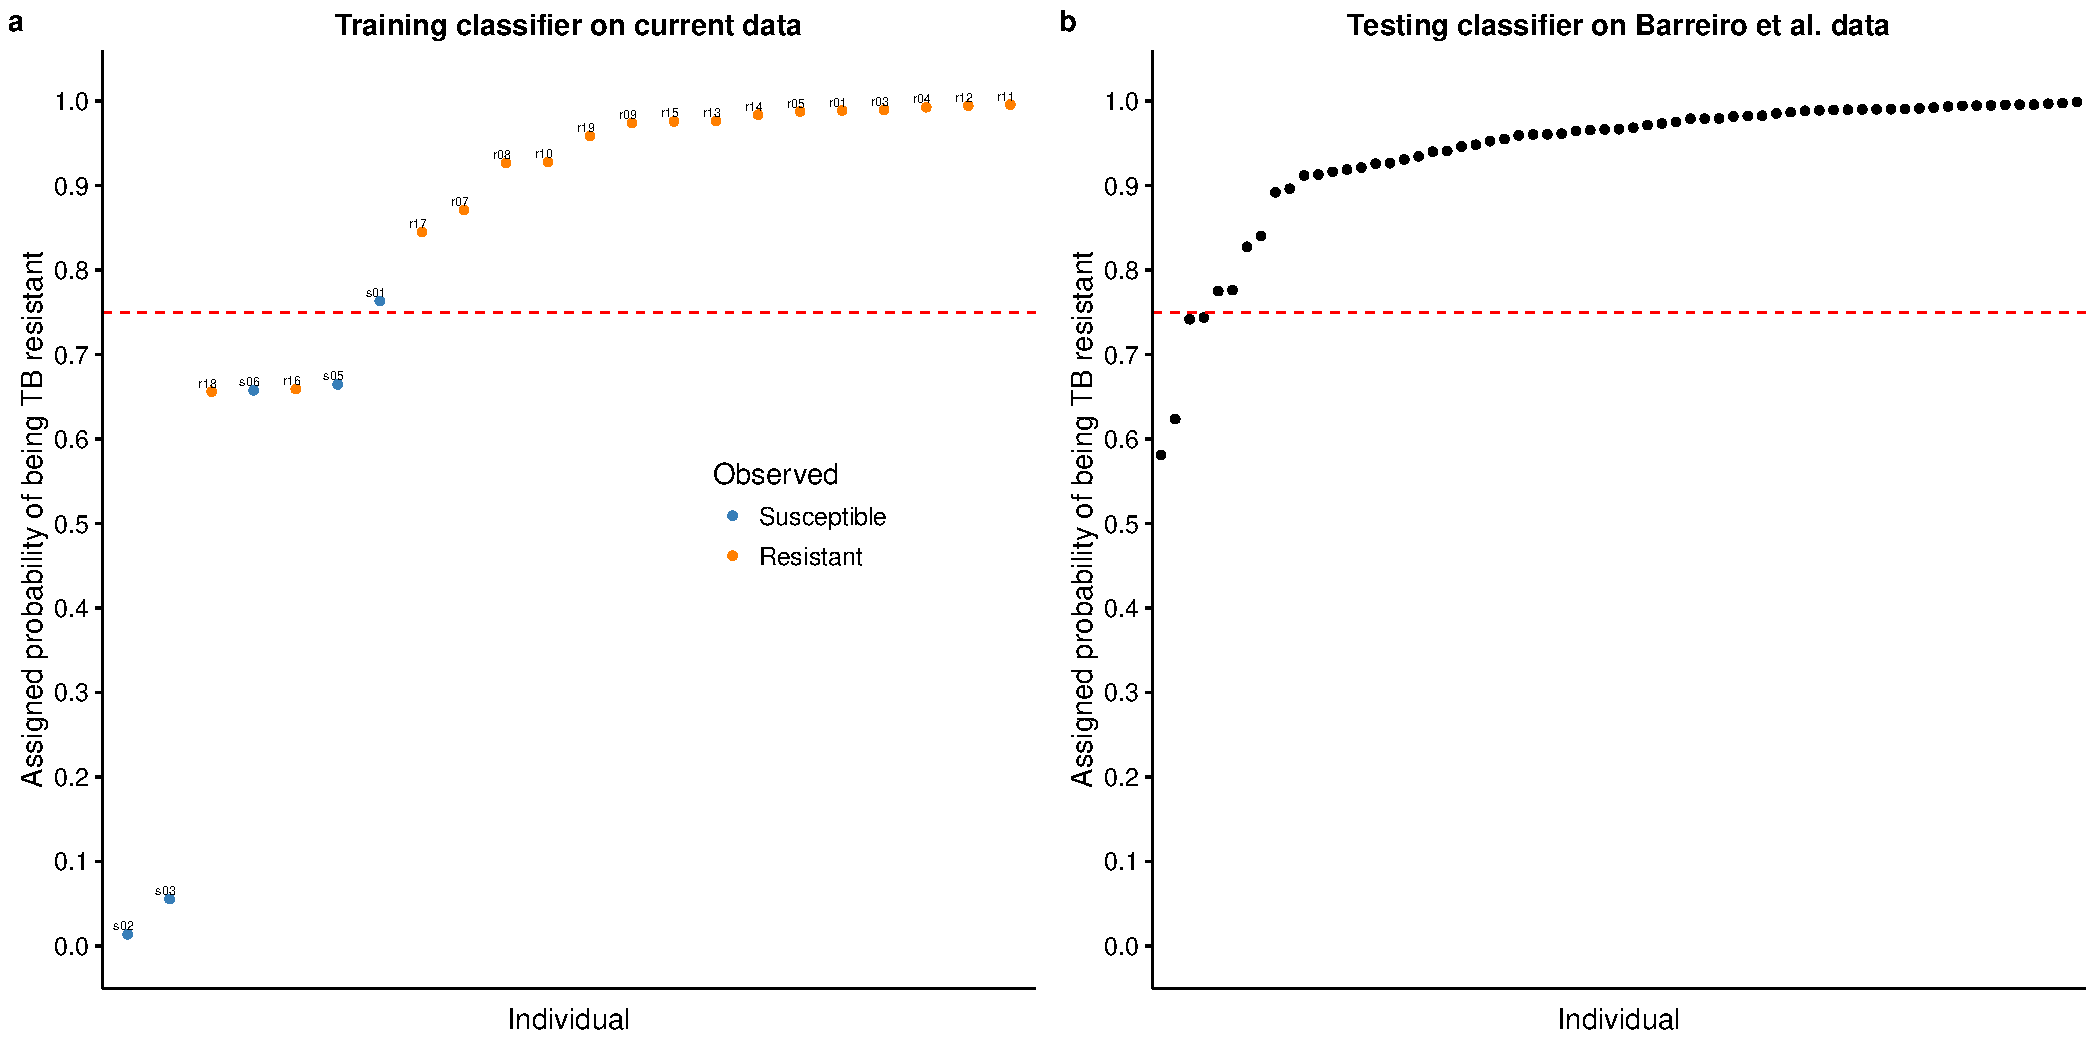
\includegraphics[width=5in]{img/ch03/classifier-en.pdf}
\caption[Classifying TB susceptible individuals using an elastic net
  model.]{ \textbf{Classifying TB susceptible individuals using an
    elastic net model.} (a) The estimates of predicted probability of
  TB resistance from the leave-one-out-cross-validation for
  individuals in the current study.  The blue circles represent
  individuals known to be susceptible to TB, and orange those
  resistant to TB. The horizontal blue line at a probability of 0.75
  almost separates susceptible and resistant individuals. (b) The
  estimates of predicted probability of TB resistance from applying
  the classifier trained on the data from the current study to a test
  set of independently collected healthy individuals
  \citep{Barreiro2012}.  }
\label{fig:class-en}
\end{figure}

\begin{figure}[!htb]
\centering 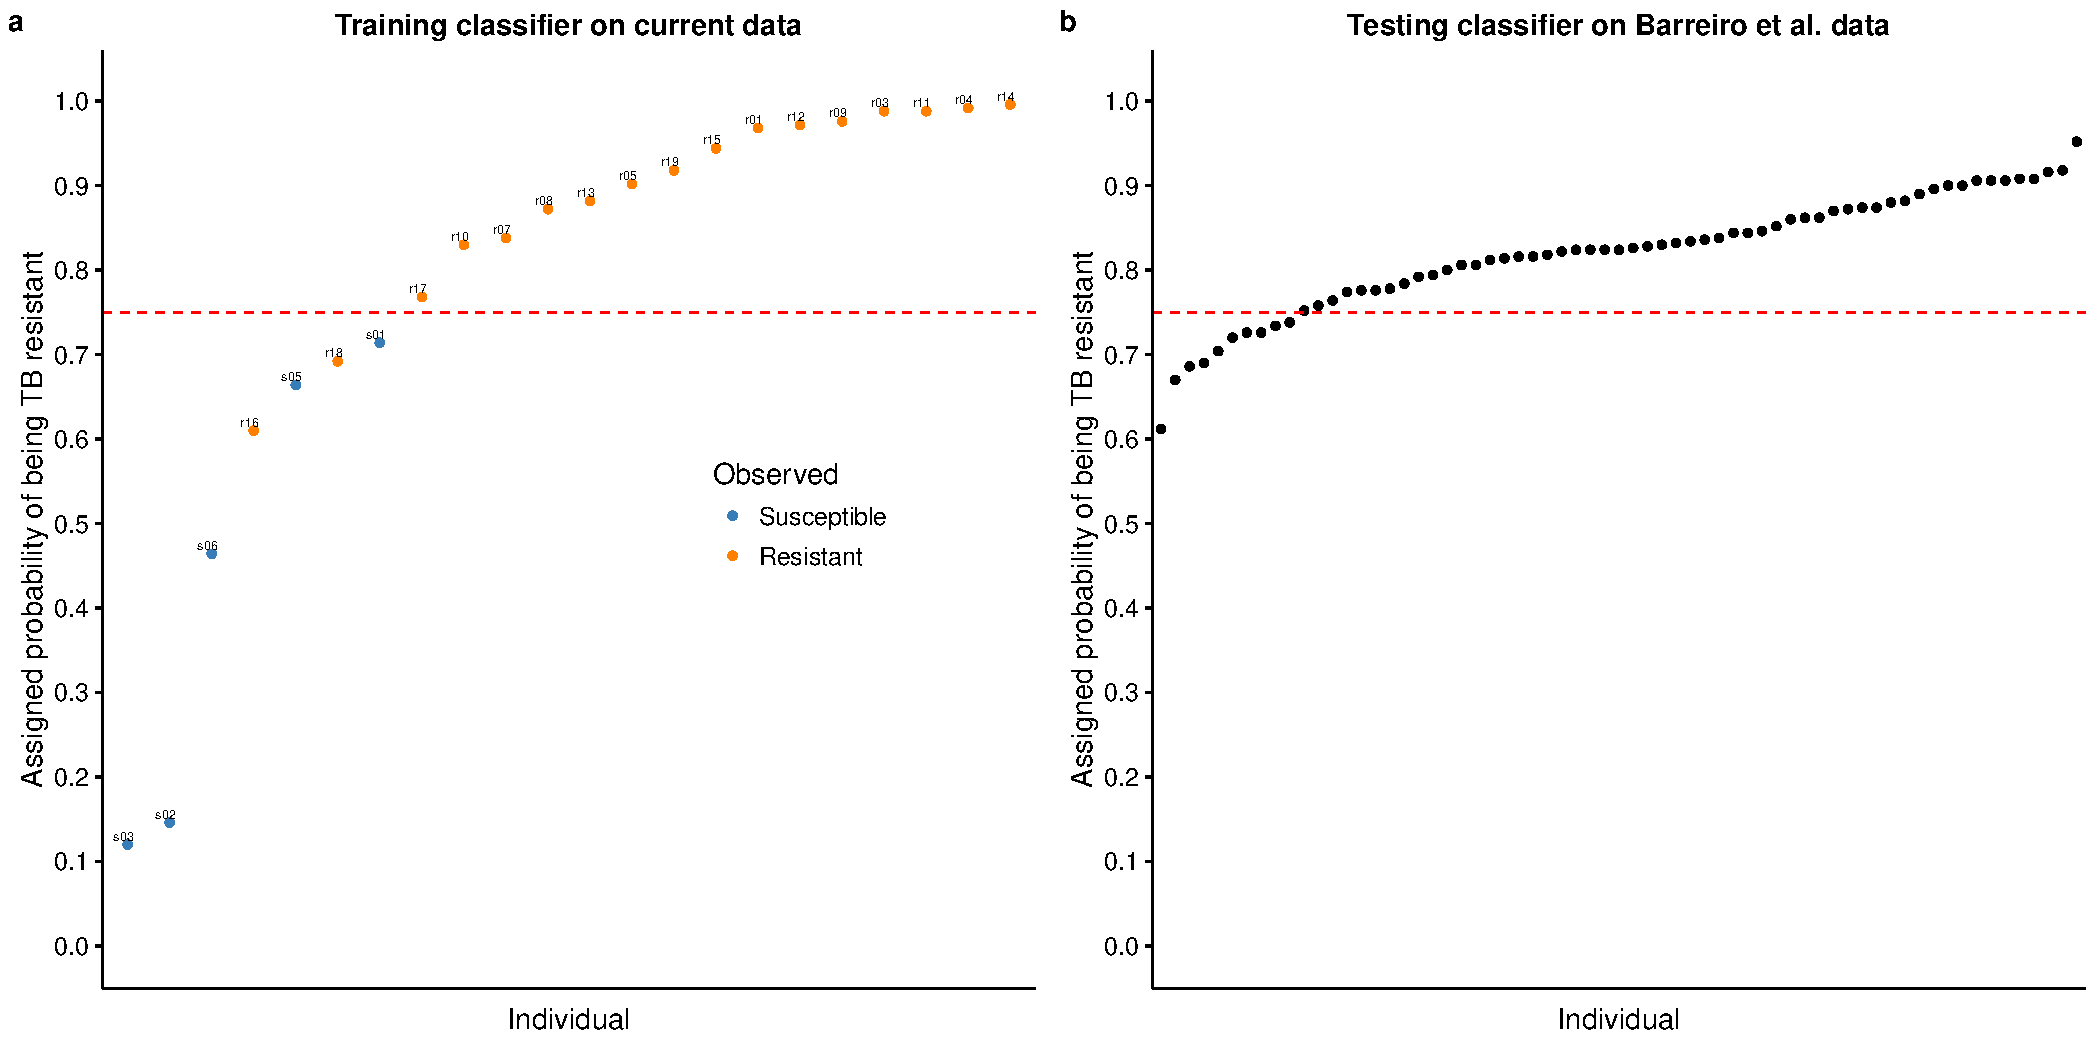
\includegraphics[width=5in]{img/ch03/classifier-rf.pdf}
\caption[Classifying TB susceptible individuals using a random forest
  model.]{ \textbf{Classifying TB susceptible individuals using a
    random forest model.}  (a) The estimates of predicted probability
  of TB resistance from the leave-one-out-cross-validation for
  individuals in the current study.  The blue circles represent
  individuals known to be susceptible to TB, and orange those
  resistant to TB. The horizontal blue line at a probability of 0.75
  separates susceptible and resistant individuals.  (b) The estimates
  of predicted probability of TB resistance from applying the
  classifier trained on the data from the current study to a test set
  of independently collected healthy individuals \citep{Barreiro2012}.
}
\label{fig:class-rf}
\end{figure}

\begin{figure}[!htb]
\centering 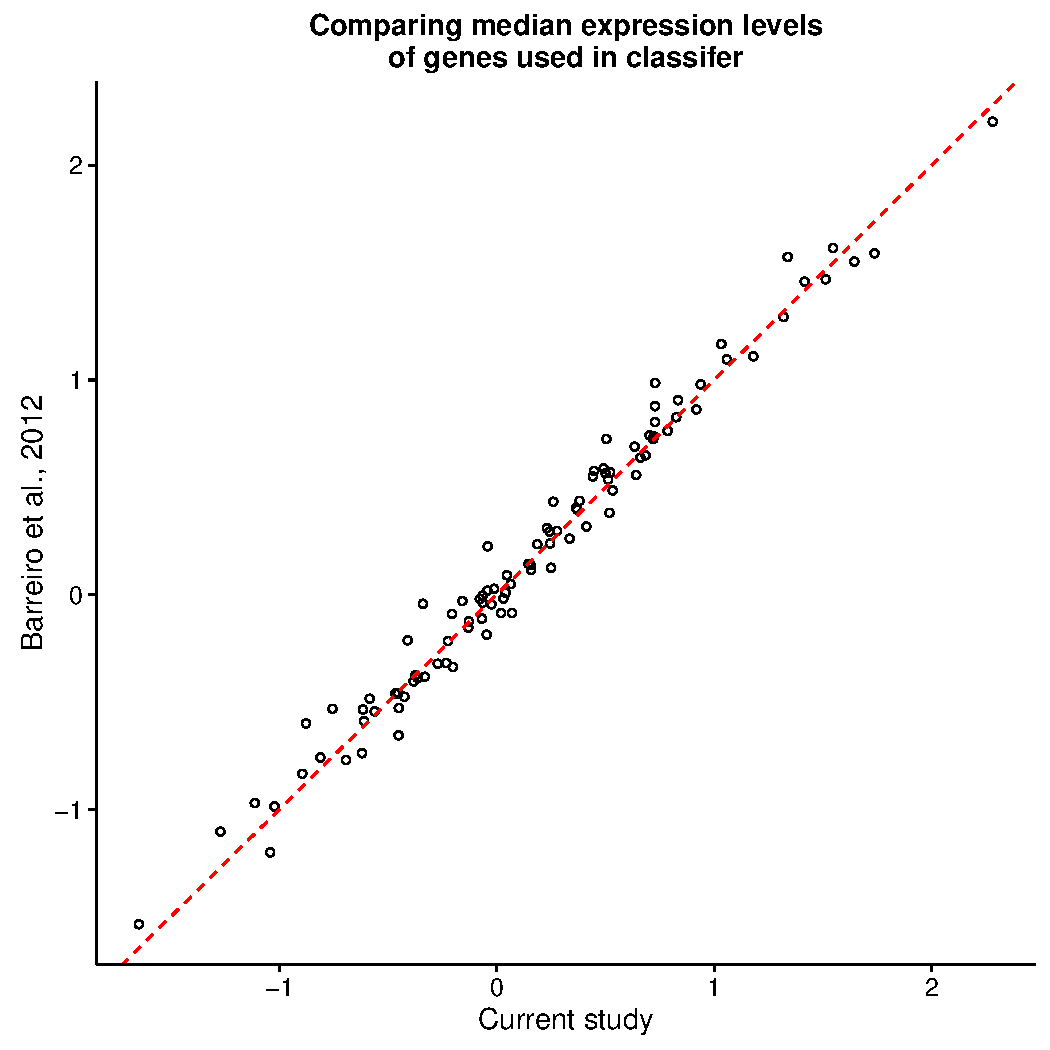
\includegraphics[width=5in]{img/ch03/classifier-exp.pdf}
\caption[Comparing gene expression between the two studies.]{
  \textbf{Comparing gene expression between the two studies.} After
  normalization and batch-correction, the median expression levels of
  the 99 genes used in the classifier were similar between the samples
  in the current study and those in Barreiro et al., 2012
  \citep{Barreiro2012}. The dashed red line is the 1:1 line.  }
\label{fig:class-exp}
\end{figure}

\clearpage
\subsection{Supplementary Data}

\begin{table}[!htb]
\caption[Sample information.]{\textbf{Sample information.}  (see
  supplementary file associated with this dissertation) Contains
  information on the 50 samples. Most variables describe the batch
  processing steps outlined in Supplementary
  Fig. \ref{fig:process}. ``id'' is a unique identifier for each
  sample, ``individual'' is the individual identifier (``s'' =
  susceptible, ``r'' = resistant), ``status'' is the susceptibility
  status, ``treatment'' is if the sample was infected or non-infected,
  ``infection'' is the date of the infection experiment (12 total),
  ``arrival'' is the identifier for the arrival batch (4 total),
  ``extraction'' is the batch for RNA extraction (5 total),
  ``master\_mix'' is the batch for library preparation (3 total),
  ``rin'' is the RNA Integrity Number from the Agilent Bioanalyzer,
  and ``outlier'' is a Boolean variable indicating if the sample was
  identified as an outlier (Supplementary Fig.  \ref{fig:outliers})
  and removed from the analysis. (txt) }
\label{ch03-s1}
\end{table}

\begin{table}[!htb]
\caption[Gene expression matrix.]{ \textbf{Gene expression matrix.}
  (see supplementary file associated with this dissertation) Contains
  the gene expression counts for the 11,336 genes after filtering
  lowly expressed genes for all 50 samples (Supplementary
  Fig. \ref{fig:gene}). Each row is a gene labeled with its Ensembl
  gene ID. Each column is a sample. Each sample is labeled according
  to the pattern ``x\#\#-status-treatment'', where x is ``r'' for
  resistant or ``s'' for susceptible, \#\# is the ID number, status is
  ``resist'' for resistant or ``suscep'' for susceptible, and
  treatment is ``noninf'' for non-infected or ``infect'' for
  infected. (txt) }
\label{ch03-s2}
\end{table}

\begin{table}[!htb]
\caption[Differential expression results.]{ \textbf{Differential
    expression results.}  (see supplementary file associated with this
  dissertation) Contains the results of the differential expression
  analysis with limma (Fig. \ref{fig:limma}). The workbook contains 4
  sheets corresponding to the 4 tests performed. ``status\_ni'' is the
  test between resistant and susceptible individuals in the
  non-infected state, ``status\_ii'' is the test between resistant and
  susceptible individuals in the infected state, ``treat\_resist'' is
  the test between the non-infected and infected states for resistant
  individuals, and ``treat\_suscep'' is the test between the
  non-infected and infected states for susceptible individuals. Each
  sheet has the same columns. ``id'' is the Ensembl gene ID, ``gene''
  is the gene name, ``logFC'' is the log fold change from limma,
  ``AveExpr'' is the average log expression from limma, ``t'' is the
  t-statistic from limma, ``P.Value'' is the p-value from limma,
  ``adj.P.Val'' is the adjusted p-value from limma, ``qvalue'' is the
  q-value calculated with adaptive shrinkage, ``chr'' is the
  chromosome where the gene is located, ``description'' is the
  description of the gene from Ensembl, ``phenotype'' is the
  associated phenotype(s) assigned my Ensembl, ``go\_id'' is the
  associated GO term(s) assigned by Ensembl, and ``go\_description''
  is the corresponding name(s) of the GO term(s). (xlsx) }
\label{ch03-s3}
\end{table}

\begin{table}[!htb]
\caption[Data for combined analysis of gene expression data and GWAS
  results.]{ \textbf{Data for combined analysis of gene expression
    data and GWAS results.}  (see supplementary file associated with
  this dissertation) Contains the results of the GWAS comparison
  analysis (Fig. \ref{fig:gwas}). The first sheet ``input-data''
  contains the data for the 10,260 genes which were assigned a SNP in
  the studies from The Gambia and Ghana. ``gwas\_p\_ghana'' is the
  minimum p-value from the GWAS in Ghana, ``gwas\_p\_gambia'' is the
  minimum p-value from the GWAS in The Gambia, and ``n\_snps'' is the
  number of GWAS SNPs within 50 kb of the transcription start
  site. The columns status\_ni, status\_ii, treat\_resist, and
  treat\_suscep refer to the tests described for Supplementary Table
  \ref{ch03-s3} and contain the absolute log fold changes for each
  comparison. All the other gene annotation columns are the same as
  described for Supplementary Table \ref{ch03-s3}. The second sheet
  ``top-genes'' contains the results of stringently filtering the
  combined differential expression and GWAS results. ``GWAS P cutoff''
  is the p-value cutoff used for both the The Gambia and Ghana GWAS,
  ``Effect size cutoff'' is the cutoff of the absolute log fold change
  for the test between susceptible and resistant individuals in the
  non-infected state (Fig. \ref{fig:limma}a), ``Number of genes'' is
  the number of genes which satisfied these thresholds, and ``Names''
  is the corresponding official gene names (sorted
  alphabetically). (xlsx) }
\label{ch03-s4}
\end{table}

\begin{table}[!htb]
\caption[Classifier results.]{ \textbf{Classifier results.}  (see
  supplementary file associated with this dissertation) Contains the
  results of the classifier analysis.  Specifically it contains the
  results from the support vector machine using the genes with a
  qvalue less than 0.05 (Fig.  \ref{fig:classifier}). The sheet
  ``gene-list'' contains information about the genes used for the
  classifier (the columns are described in the section for
  Supplementary Table \ref{ch03-s3}). The sheet ``training-input''
  contains the input gene expression data for training the model. The
  sheet ``training-results'' contains the results of the
  leave-one-out-cross-validation when training the model on the
  samples from the current study.  The sheet ``testing-input''
  contains the input gene expression data for testing the model. The
  sheet ``testing-results'' contains the results from testing the
  model on the samples from Barreiro et al., 2012
  \citep{Barreiro2012}. The column ``prob\_tb\_resist'' is the
  probability of being resistant to TB assigned by the model. (xlsx) }
\label{ch03-s5}
\end{table}
